% !TEX root = ../thesis.tex

\section{$V$-tagging Scale Factors}
\label{sec:vTag}

% Deriving scale factors
As mentioned previously, the top-enriched control region is obtained by inverting the $b$-tag veto, thereby requiring the presence of at least one $b$-tagged jet in the event.
The region is used to calibrate the performance of the soft drop algorithm and jet substructure variables on merged bosons.
In particular, the scale factors for the $V$-tagging selection in the HP and LP categories are derived in this region using a dedicated fit of the soft drop jet mass spectrum.
We also include events with $\nsubjDDT>0.80$ as a separate category denoted by NP to avoid bias resulting from only selecting HP and LP events.
This allows us to accurately model the $W^\pm$ peak for all categories used in the analysis.

\subsection{Fit Model}

% Fit model
Our fit model relies on two classes of events in the top-enriched region.
The first corresponds to resonant $W^\pm$ events that are the result of a top decay, with the $b$ jet outside of the AK8 jet.
The second class consists of non-resonant events resulting from random combinations of a merged AK8 jet.
To account for both of these types of events, we employ a fit model that uses a double crystal ball (DCB) for the $W^\pm$, another DCB for the partially reconstructed top quark, an exponential, and a uniform distribution.
Once the fit is performed, we then merge the second DCB, exponential, and uniform distributions to form a single non-resonant shape.

% Crystal ball function
The crystal ball function is a composite function consisting of a power-law stitched to a Gaussian core~\cite{Cheng_2016}, defined by
\begin{equation}
  f_\mathrm{CB}(x;\mu,\sigma,\alpha,n)=N
  \begin{cases}
    e^{-\frac{1}{2}\pqty{\frac{x-\mu}{\sigma}}^2}, & \frac{x-\mu}{\sigma}>-\alpha,\\
    \pqty{\frac{n}{|\alpha|}}^ne^{-\frac{|\alpha|^2}{2}}\pqty{\frac{n}{|\alpha|}-|\alpha|-\frac{x-\mu}{\sigma}}^{-n} & \frac{x-\mu}{\sigma}\leq-\alpha,
  \end{cases}
\end{equation}
where $\alpha$ is a parameter that determines the cutoff between the Gaussian core and the powertail, $n$ is the exponent of the powertail, and $N$ is a normalization factor.
The double crystal ball instead has powertails on both sides of the Gaussian core, and is given by
\begin{equation}
  f_\mathrm{DCB}(x;\mu,\sigma,\alpha_1,\alpha_2,n_1,n_2)=N
  \begin{cases}
    \pqty{\frac{n_1}{|\alpha_1|}}^{n_1}e^{-\frac{|\alpha_1|^2}{2}}\pqty{\frac{n_1}{|\alpha_1|}-|\alpha_1|-\frac{x-\mu}{\sigma}}^{-n_1} & \frac{x-\mu}{\sigma}\leq-\alpha_1,\\
    e^{-\frac{1}{2}\pqty{\frac{x-\mu}{\sigma}}^2}, & -\alpha_1<\frac{x-\mu}{\sigma}<\alpha_2,\\
    \pqty{\frac{n_2}{|\alpha_2|}}^{n_2}e^{-\frac{|\alpha_2|^2}{2}}\pqty{\frac{n_2}{|\alpha_2|}-|\alpha_2|-\frac{x-\mu}{\sigma}}^{-n_2} & \frac{x-\mu}{\sigma}\geq\alpha_2,
  \end{cases}
\end{equation}
where $\alpha_1$ and $n_1$ are the powertail parameters for the left side of the tail, and $\alpha_2$ and $n_2$ are the powertail parameters for the right side of the tail.

% Normalization
The explicit form of the fit model $f$ in each category (HP, LP, NP) is given by
\begin{align}
  & f(\mathrm{HP})=rSF^\mathrm{HP}N_W^\mathrm{HP}f_W^\mathrm{HP}+N_{NR}^\mathrm{HP}f_{NR}^\mathrm{HP},\label{eq:VtagFit1}\\
  & f(\mathrm{LP})=rSF^\mathrm{LP}N_W^\mathrm{LP}f_W^\mathrm{LP}+N_{NR}^\mathrm{LP}f_{NR}^\mathrm{LP},\label{eq:VtagFit2}\\
  & f(\mathrm{NP})=r\bqty{N_\mathrm{Total}-SF^\mathrm{HP}N_W^\mathrm{HP}-SF^\mathrm{LP}N_W^\mathrm{LP}}f_W^\mathrm{NP}+N_{NR}^\mathrm{NP}+f_{NR}^\mathrm{NP},\label{eq:VtagFit3}
\end{align}
where $f_W$ is the resonant distribution for the $W^\pm$ jet, $f_{NR}$ is the non-resonant shape, $r$ is a global scale factor accounting for lepton efficiency and luminosity, $N_{W}^\mathrm{HP}$, $N_{W}^\mathrm{LP}$, $N_{W}^\mathrm{NP}$, and $N_\mathrm{Total}$ are the number of expected events in simulation for all three categories and the total number of events, and the $SF$ are scale factors for the HP and LP categories.
This normalization is chosen to account for migration between categories.

\subsection{Fit Results}

% Fit results
We perform the fit of equations~\ref{eq:VtagFit1}-\ref{eq:VtagFit3} in a jet mass window of 20-$145\unit{GeV}$.
The resulting post-fit distributions for all three years and the full Run 2 dataset and MC samples can be seen in figure~\ref{fig:VTag_postfit_Run2}.
Table~\ref{tab:VTagFactors} shows the $V$-tagging scale factors in the HP and LP categories obtained by the fit for all years and the full Run 2 dataset, and table~\ref{tab:VScaleRes} shows the scale factors for the jet mass scale and resolution again for all years and for the full Run 2 dataset.
For the analysis we use the Run 2 scale factors in the computation of the expected signal normalizations, and the Run 2 uncertainties are used as a flat systematic uncertainty for the signal normalizations.
The scale factors for the jet mass scale and resolution are used as corrections to the signal shapes and $W^\pm$ peak for the resonant background templates.

\begin{figure}[htbp]
  \centering
  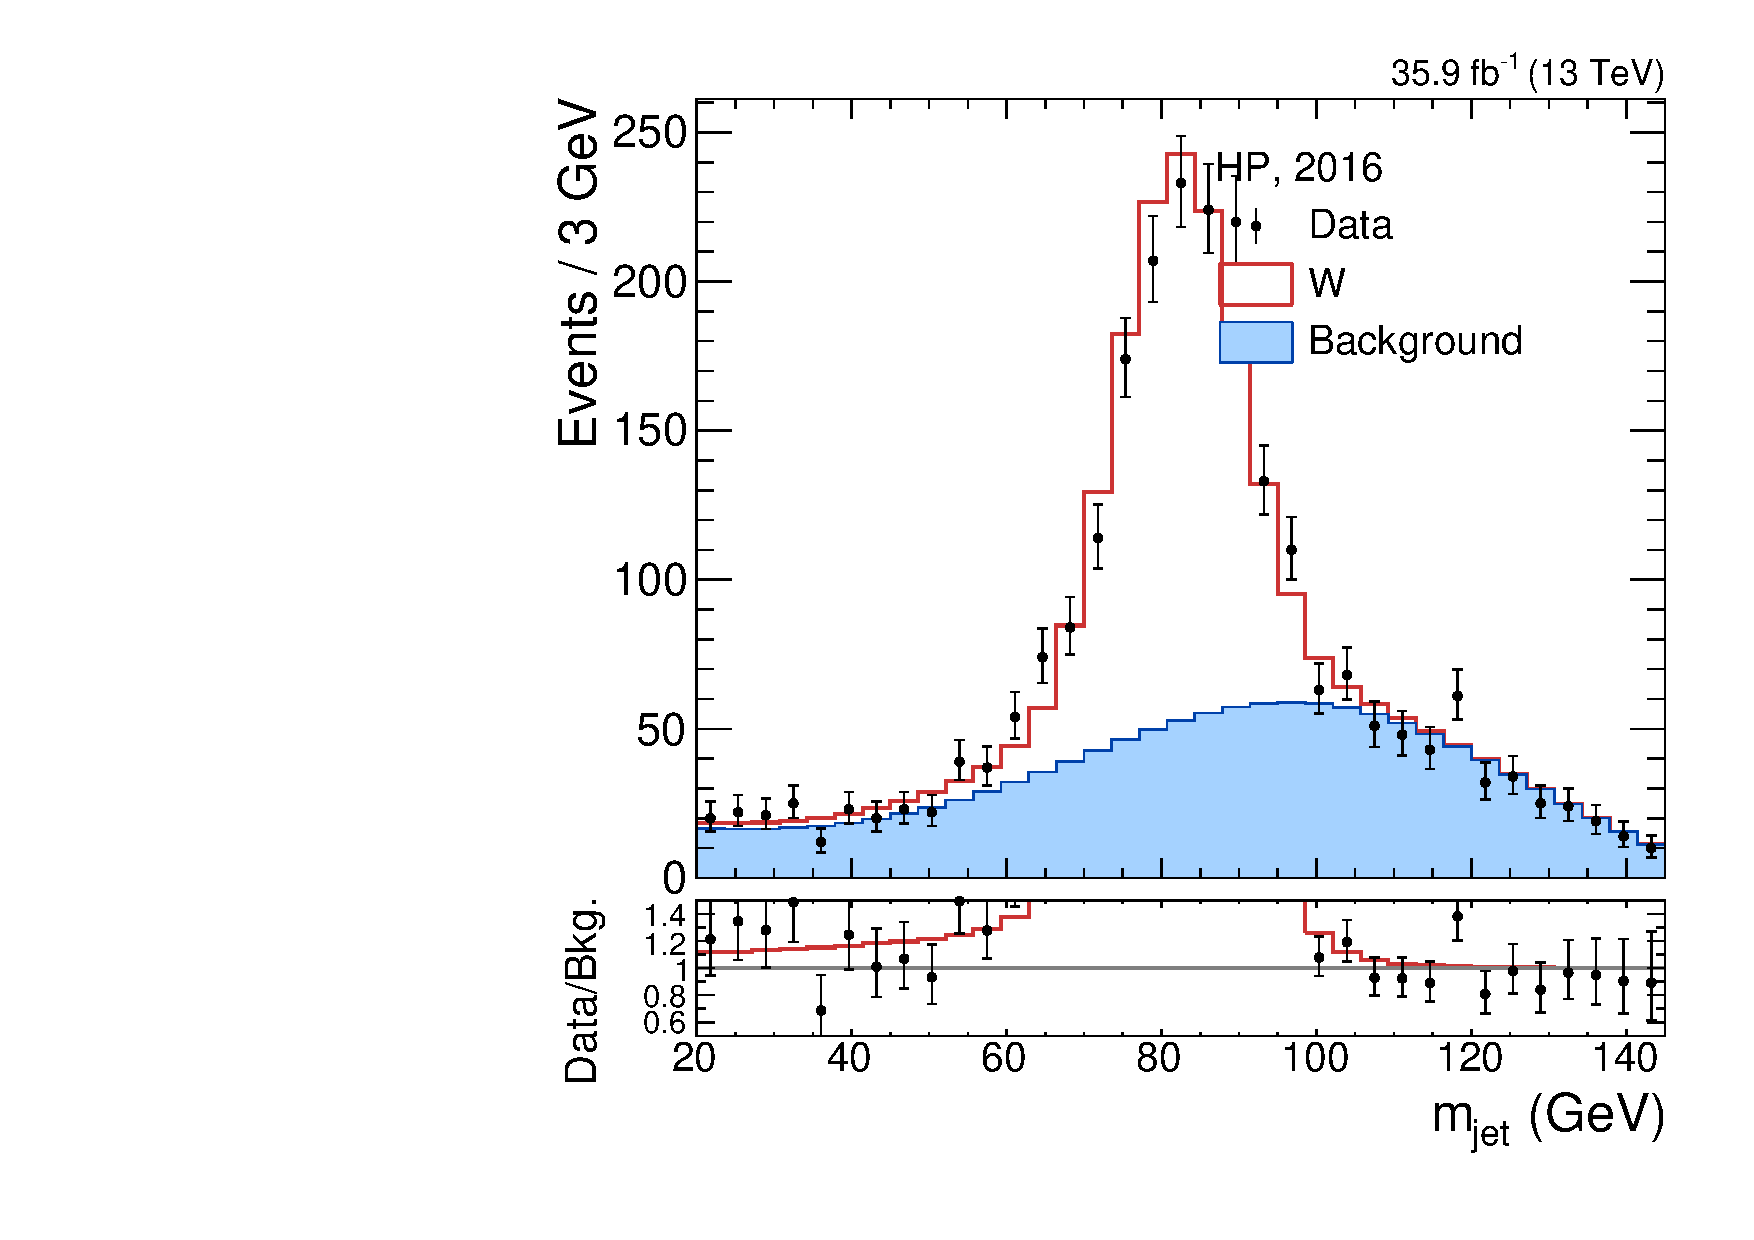
\includegraphics[width=0.3\textwidth]{fig/Vtag/PostFit__MJJ__allC_allL_HP_2016.pdf}
  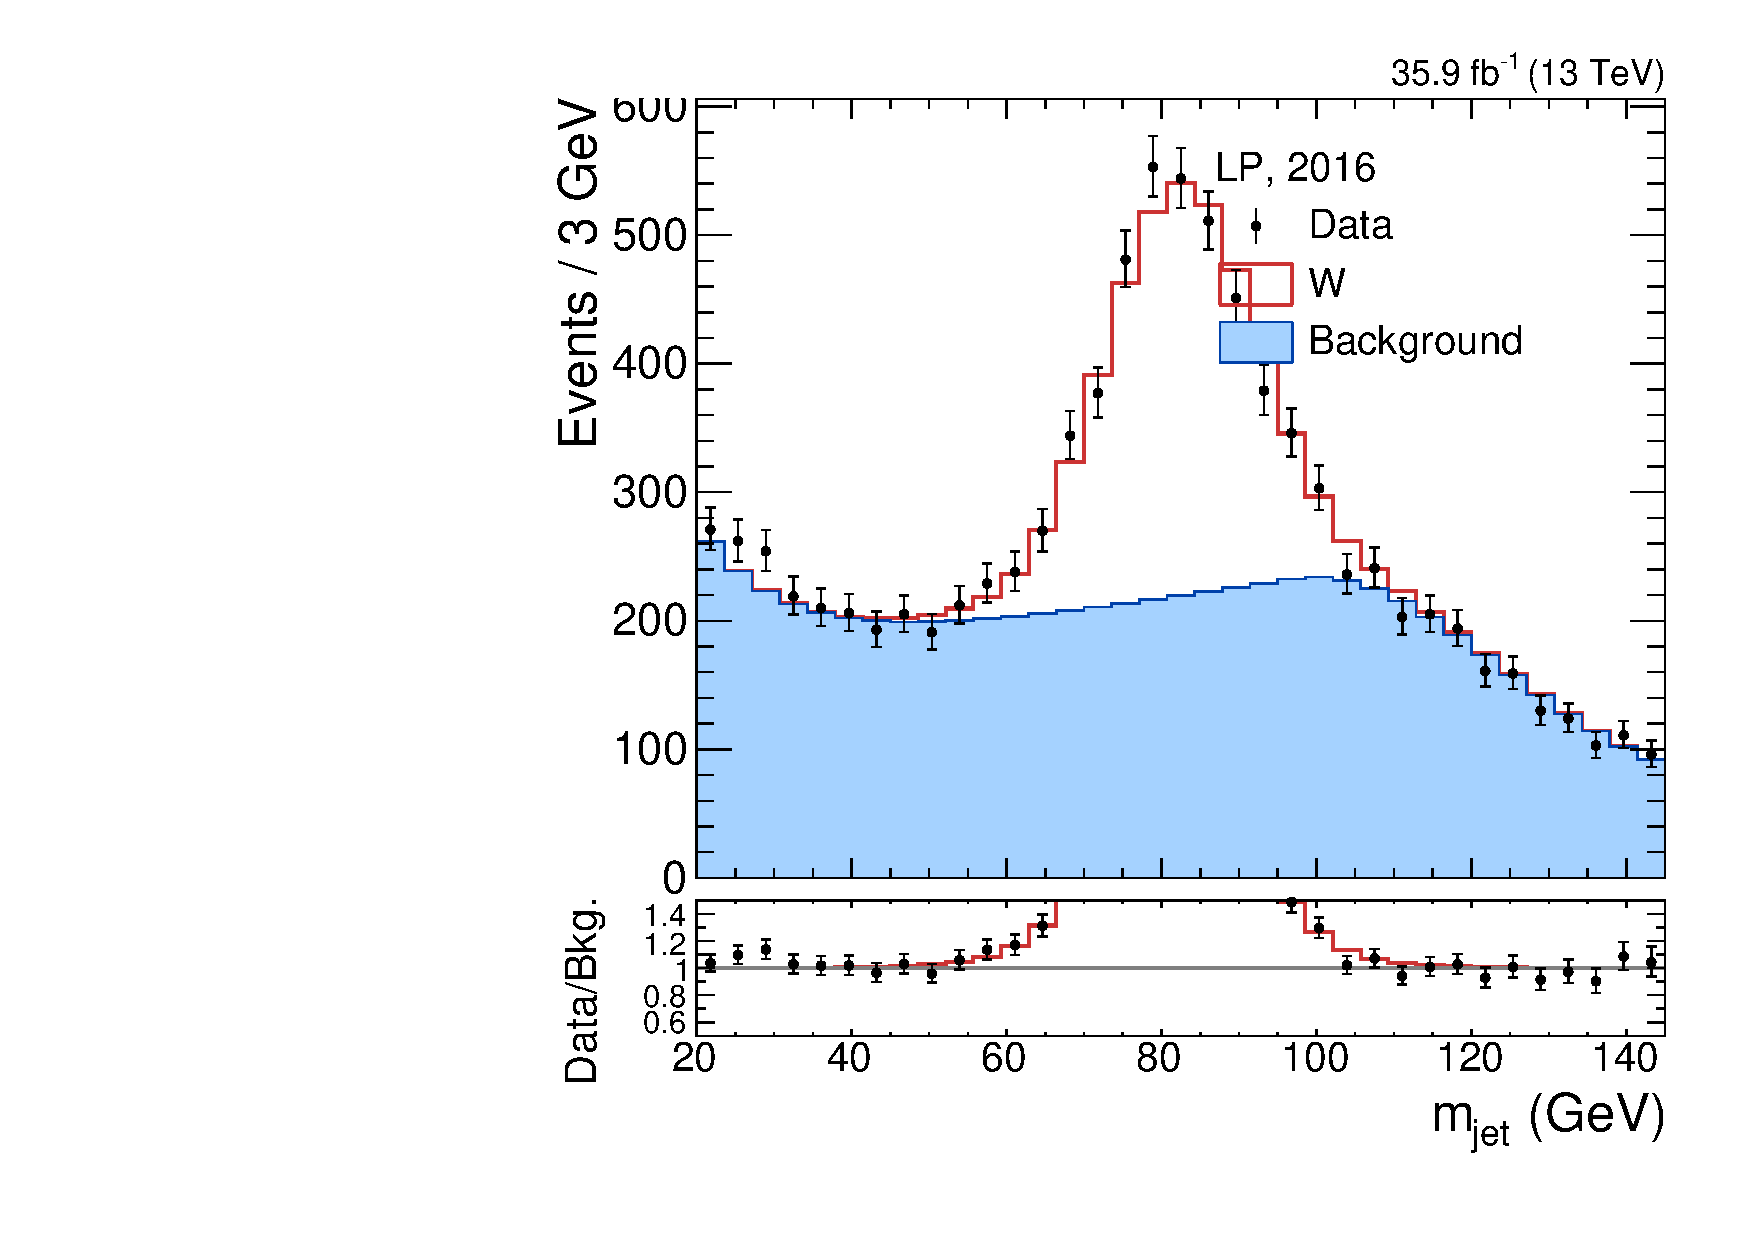
\includegraphics[width=0.3\textwidth]{fig/Vtag/PostFit__MJJ__allC_allL_LP_2016.pdf}
  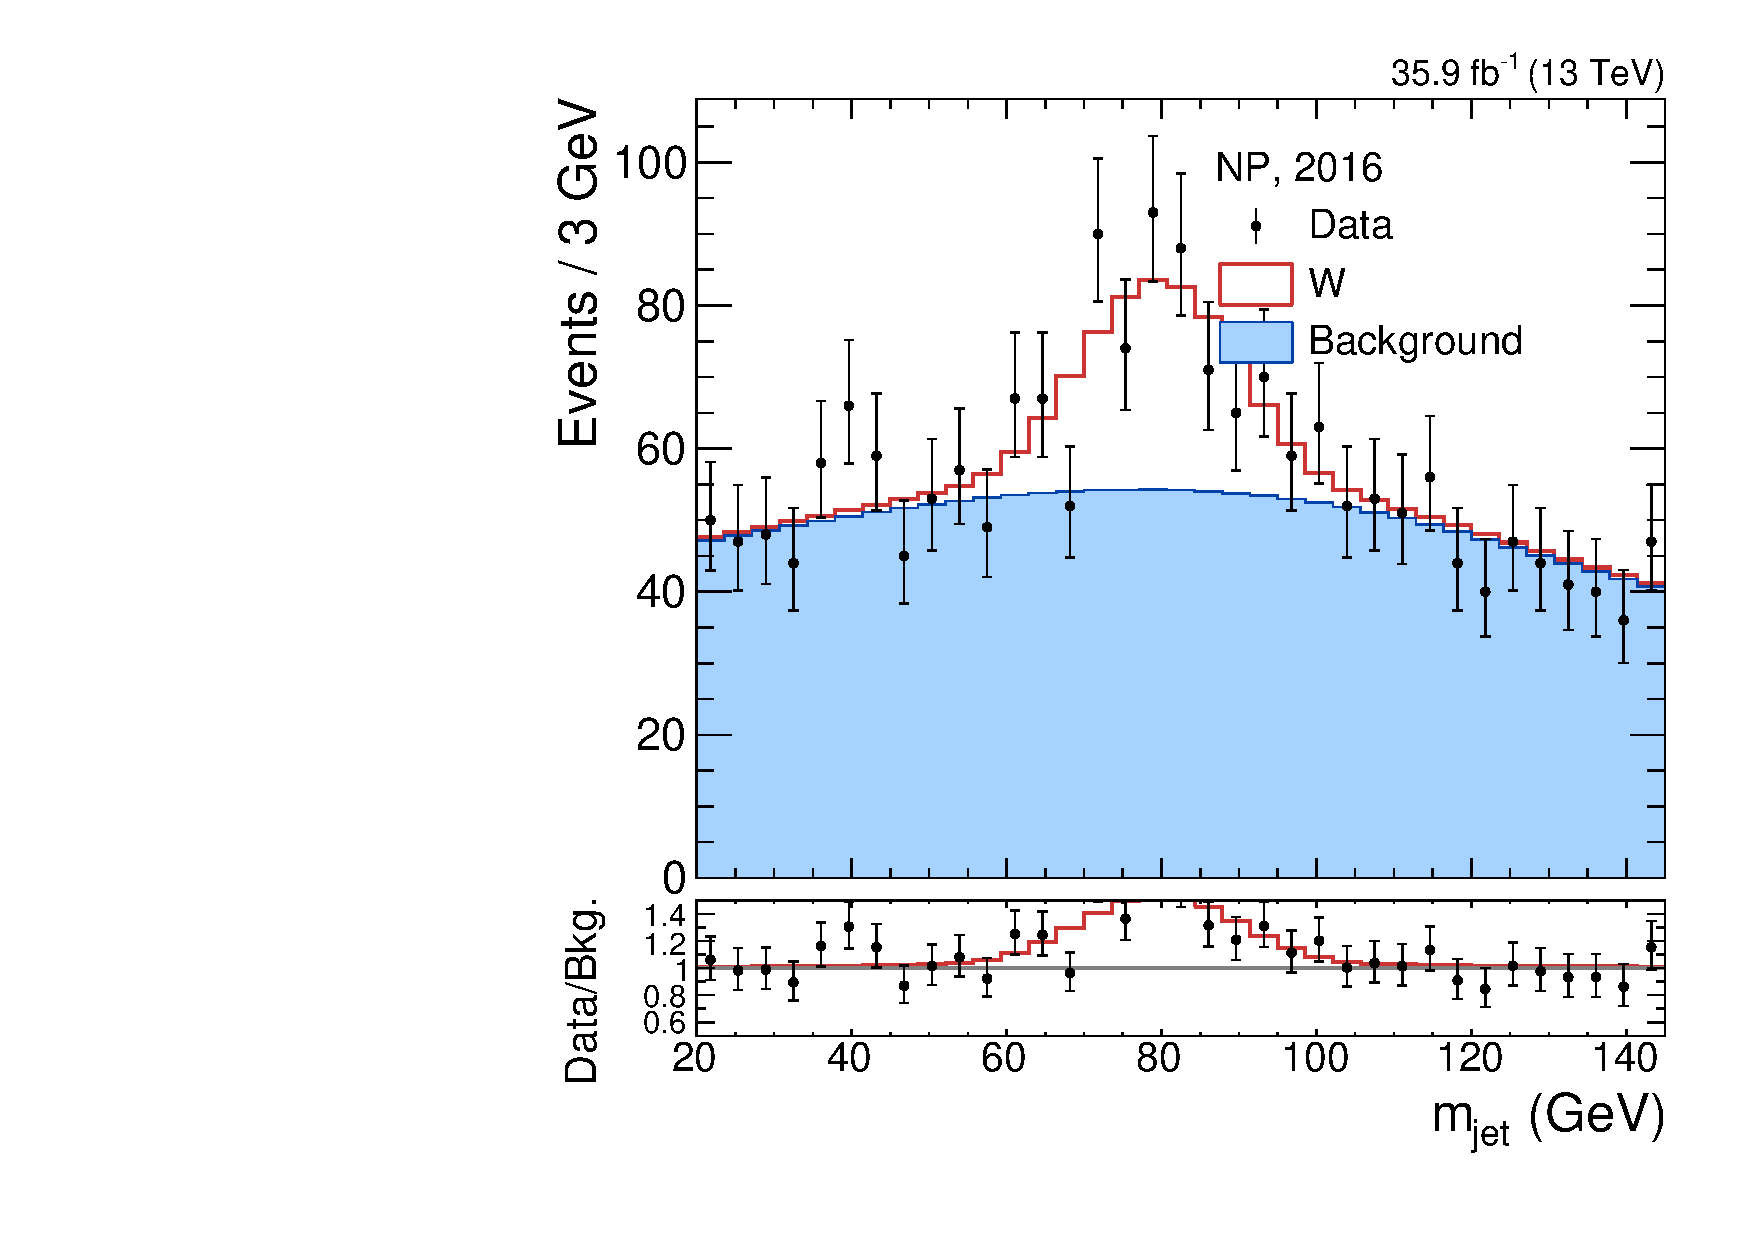
\includegraphics[width=0.3\textwidth]{fig/Vtag/PostFit__MJJ__allC_allL_NP_2016.pdf}\\
  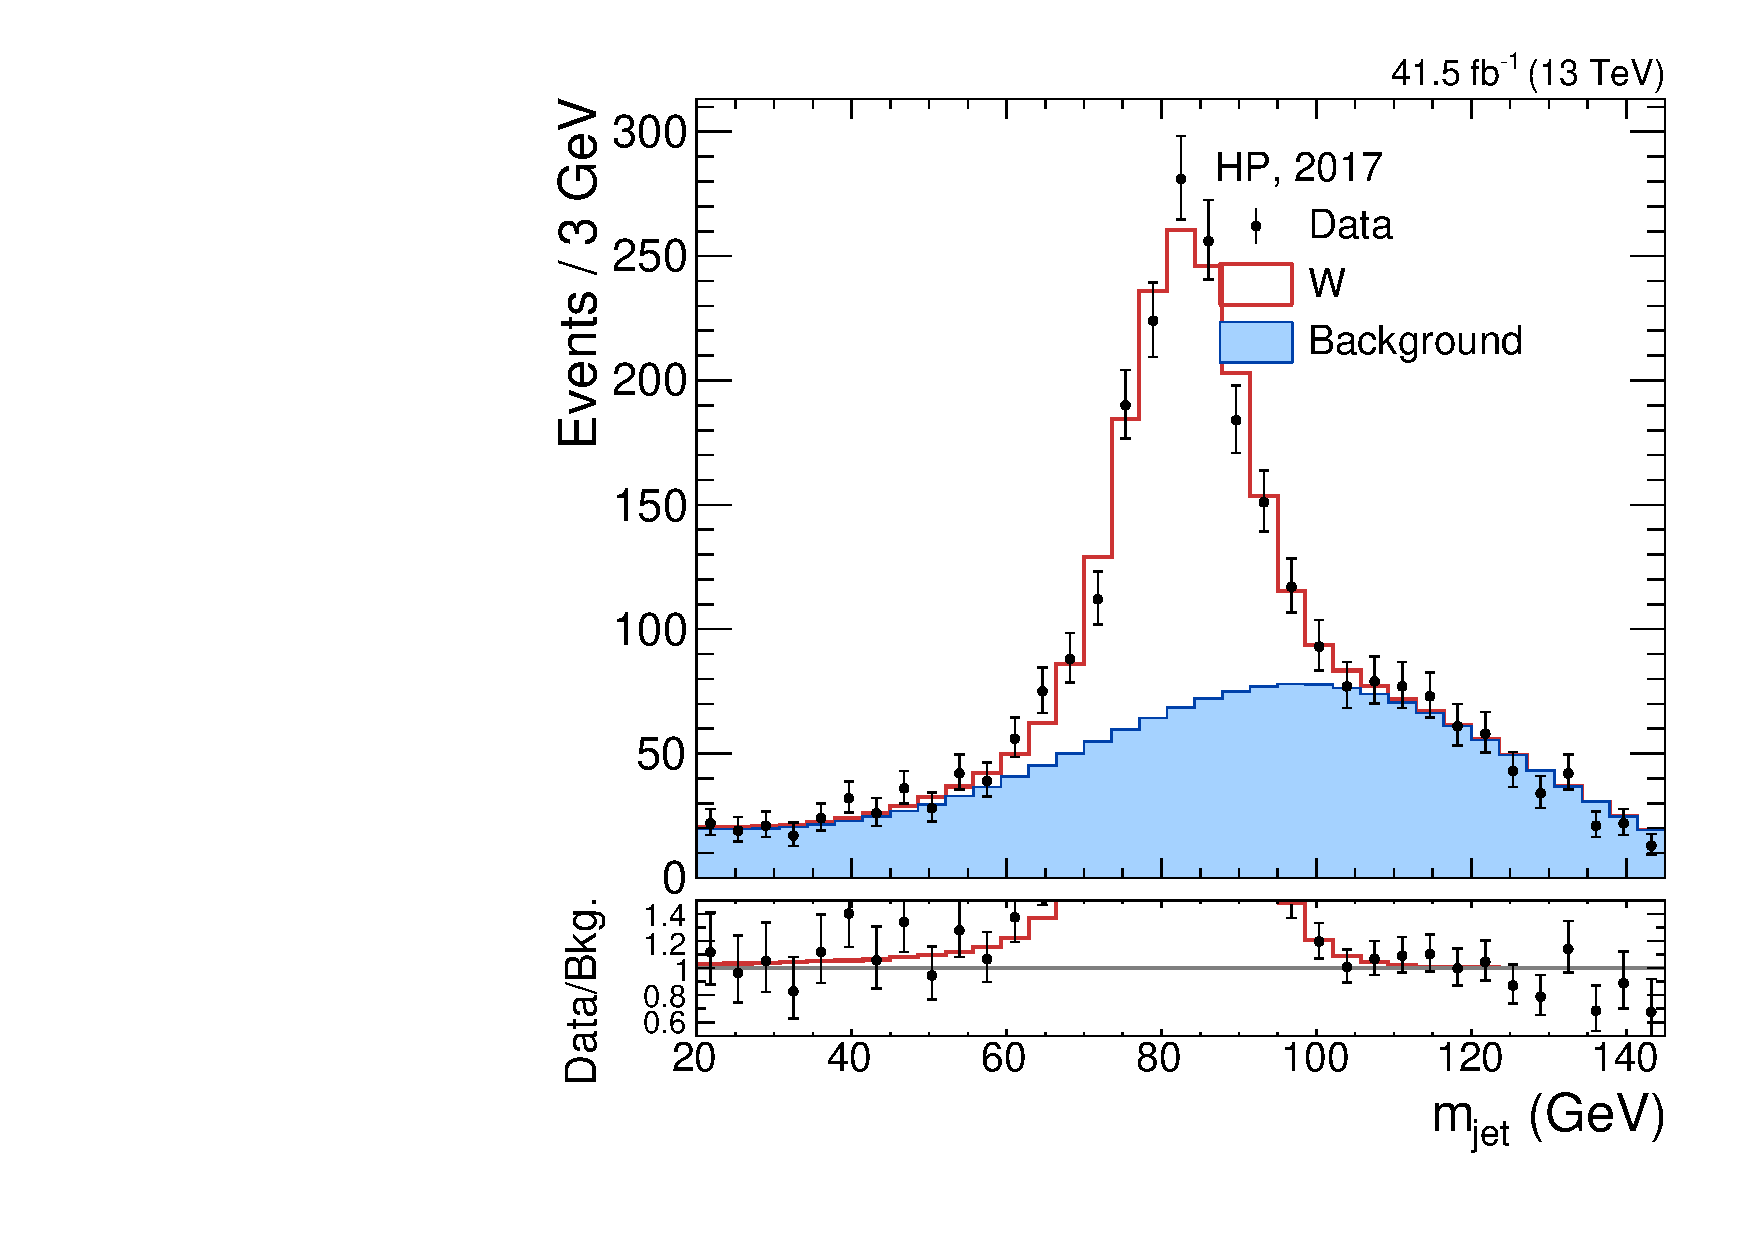
\includegraphics[width=0.3\textwidth]{fig/Vtag/PostFit__MJJ__allC_allL_HP_2017.pdf}
  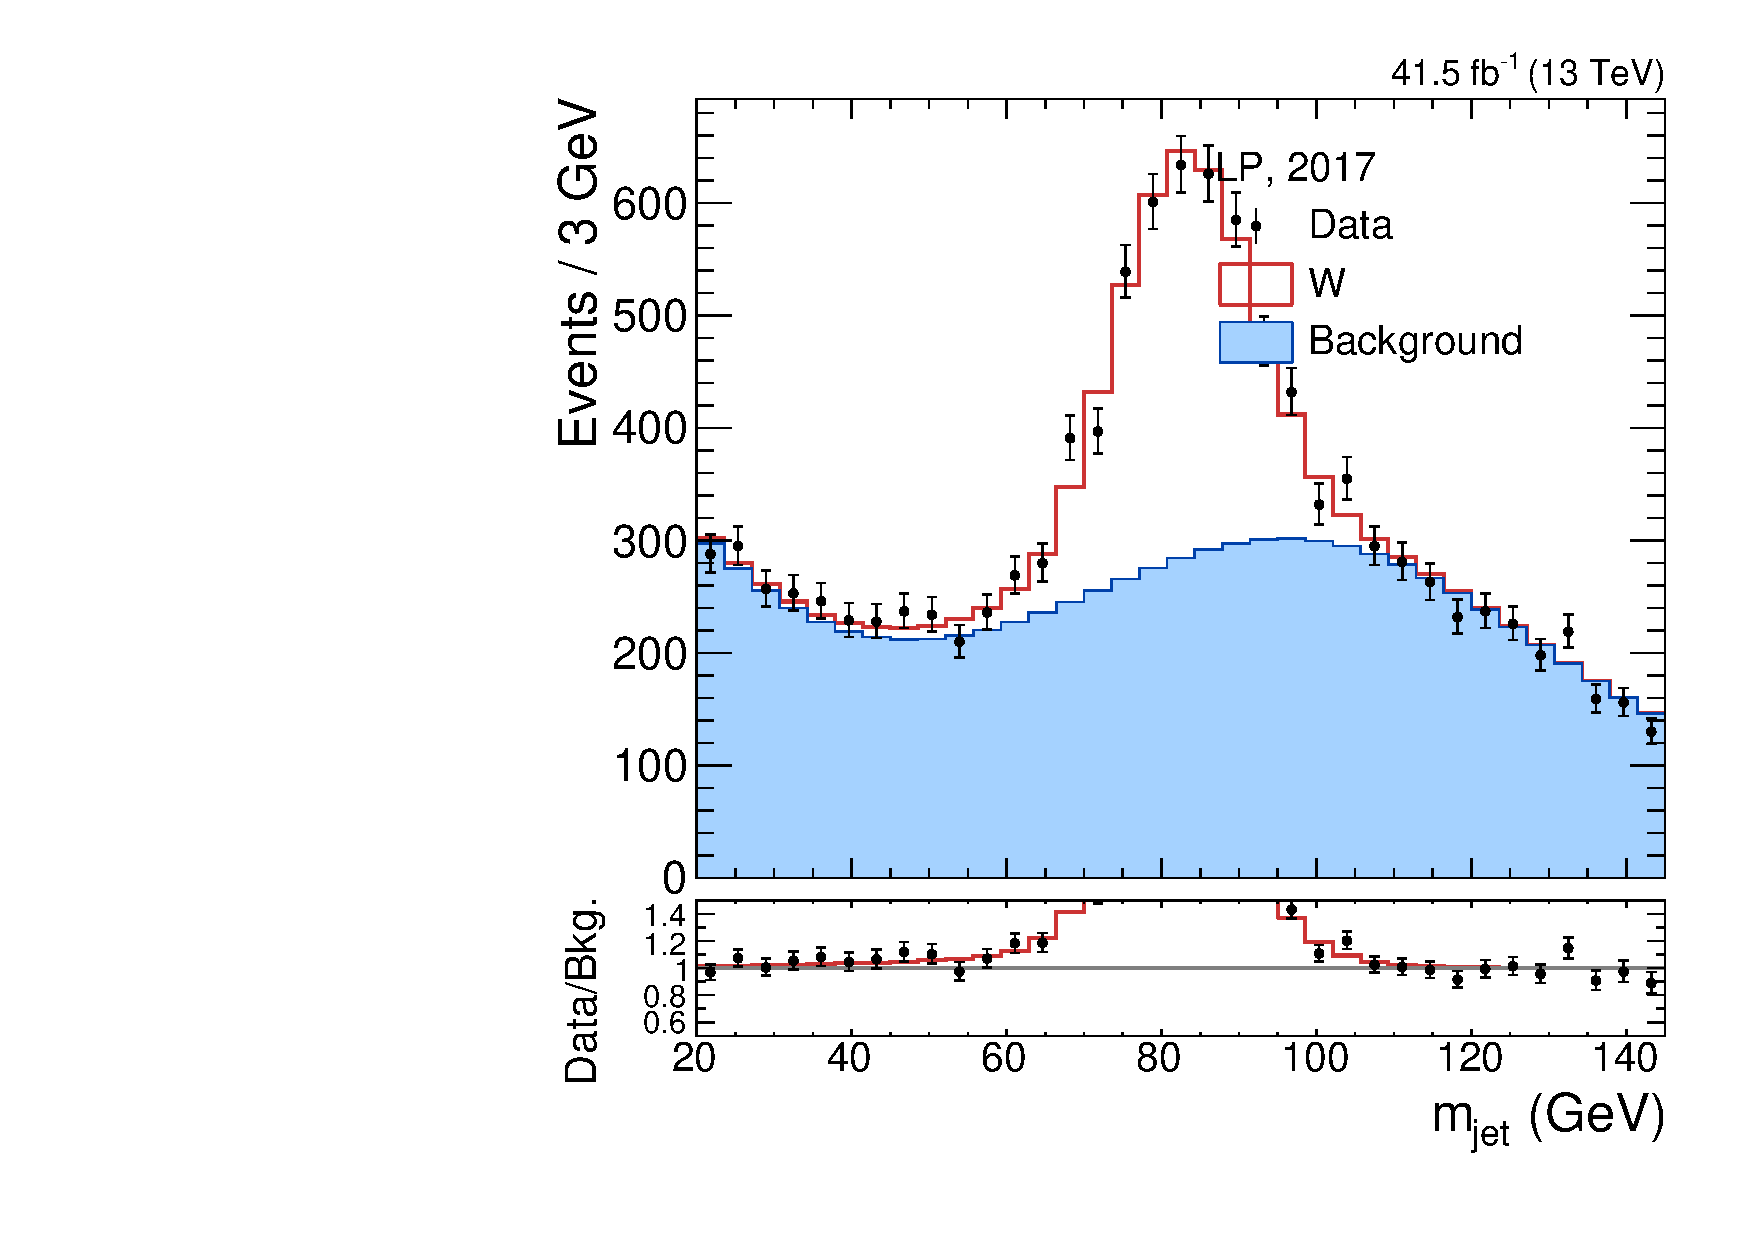
\includegraphics[width=0.3\textwidth]{fig/Vtag/PostFit__MJJ__allC_allL_LP_2017.pdf}
  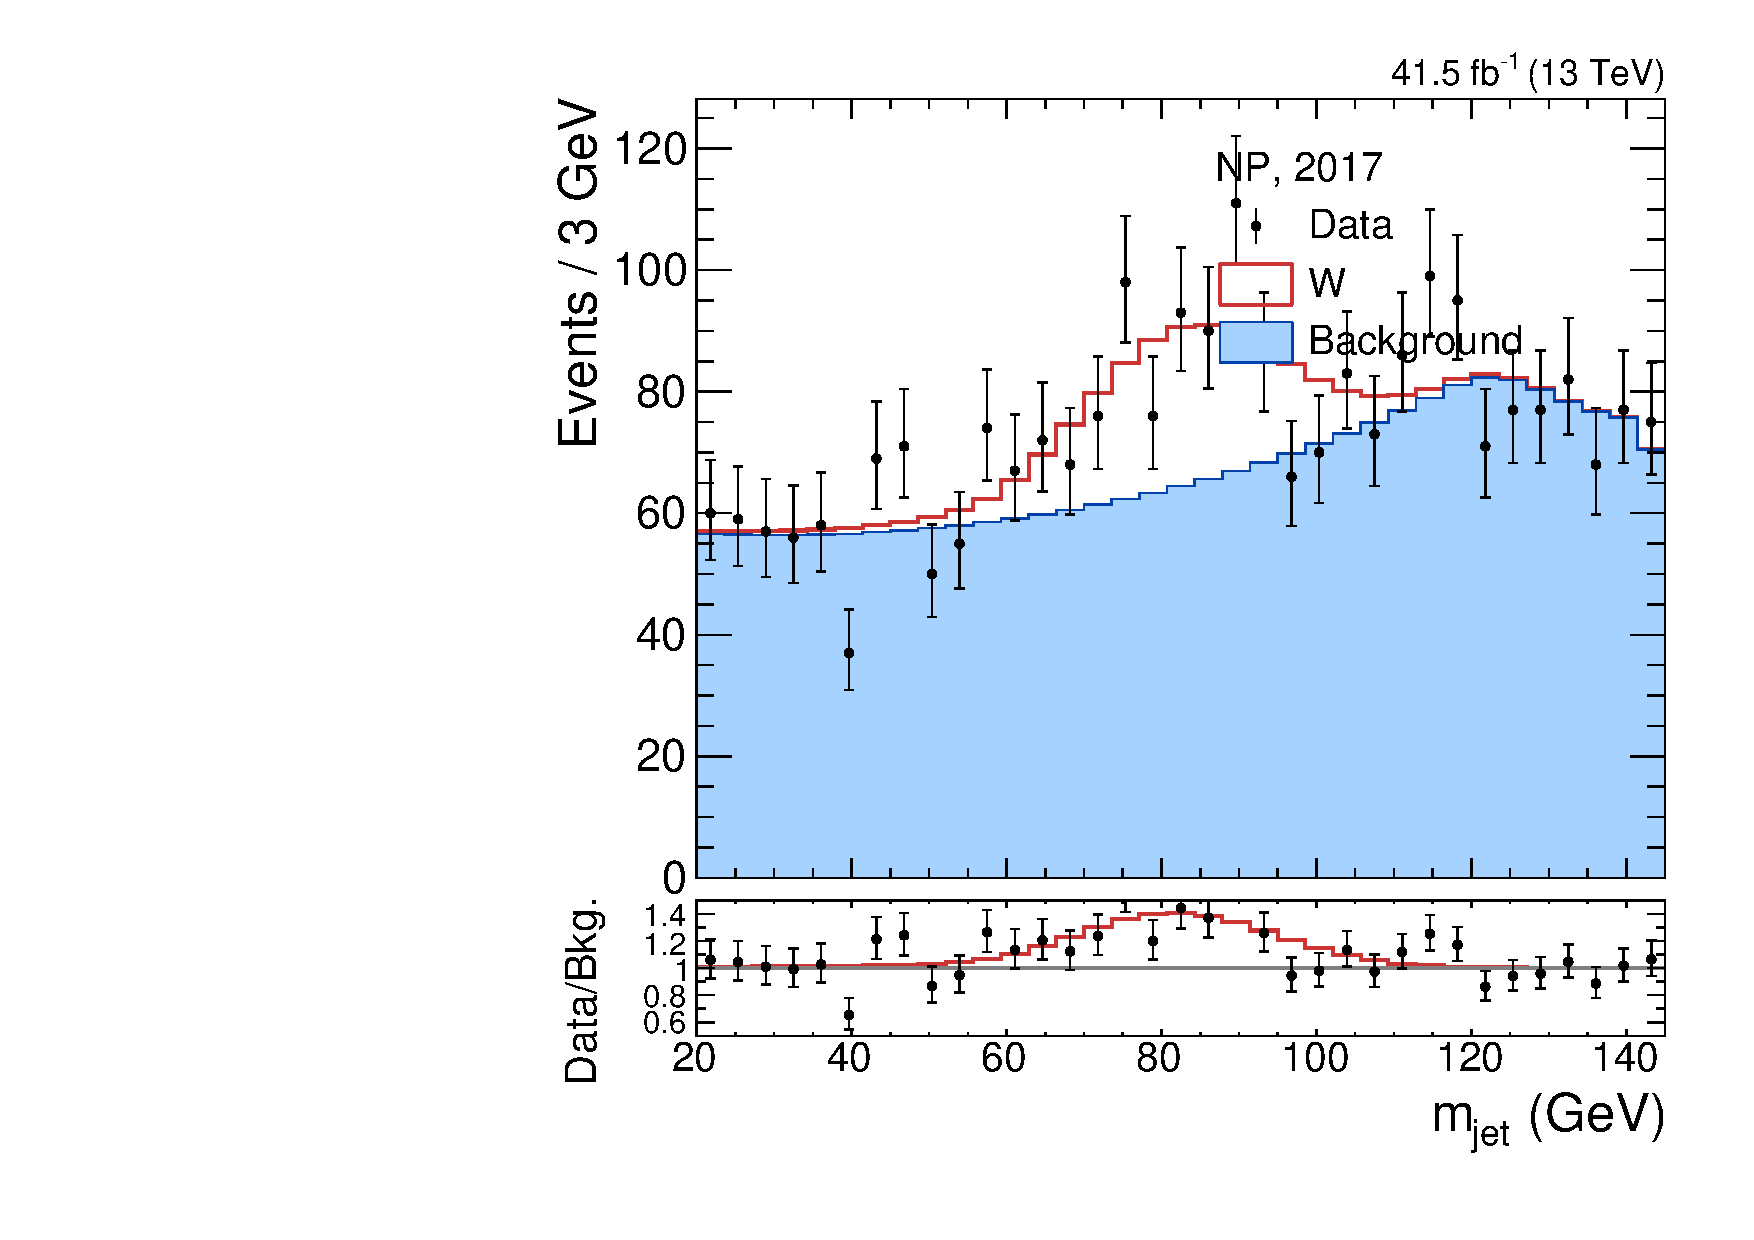
\includegraphics[width=0.3\textwidth]{fig/Vtag/PostFit__MJJ__allC_allL_NP_2017.pdf}\\
  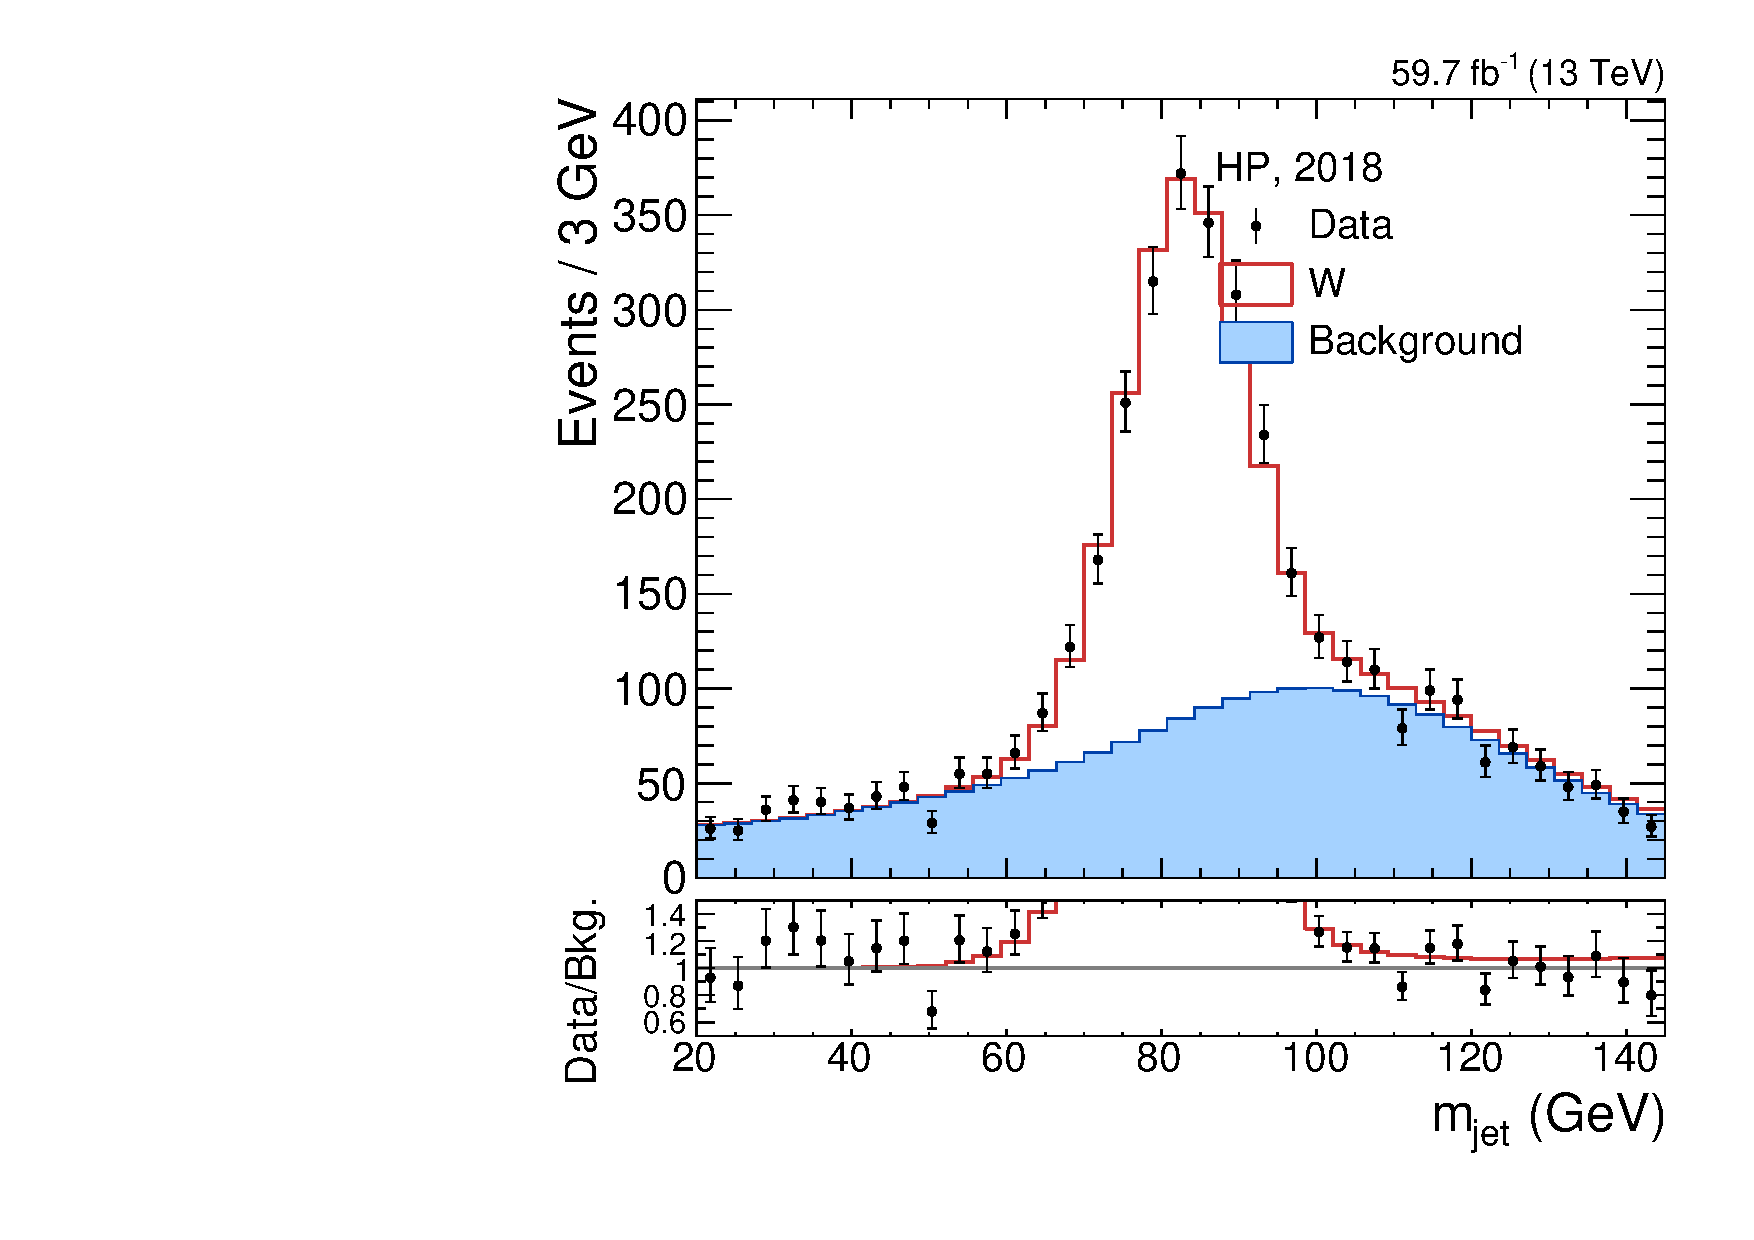
\includegraphics[width=0.3\textwidth]{fig/Vtag/PostFit__MJJ__allC_allL_HP_2018.pdf}
  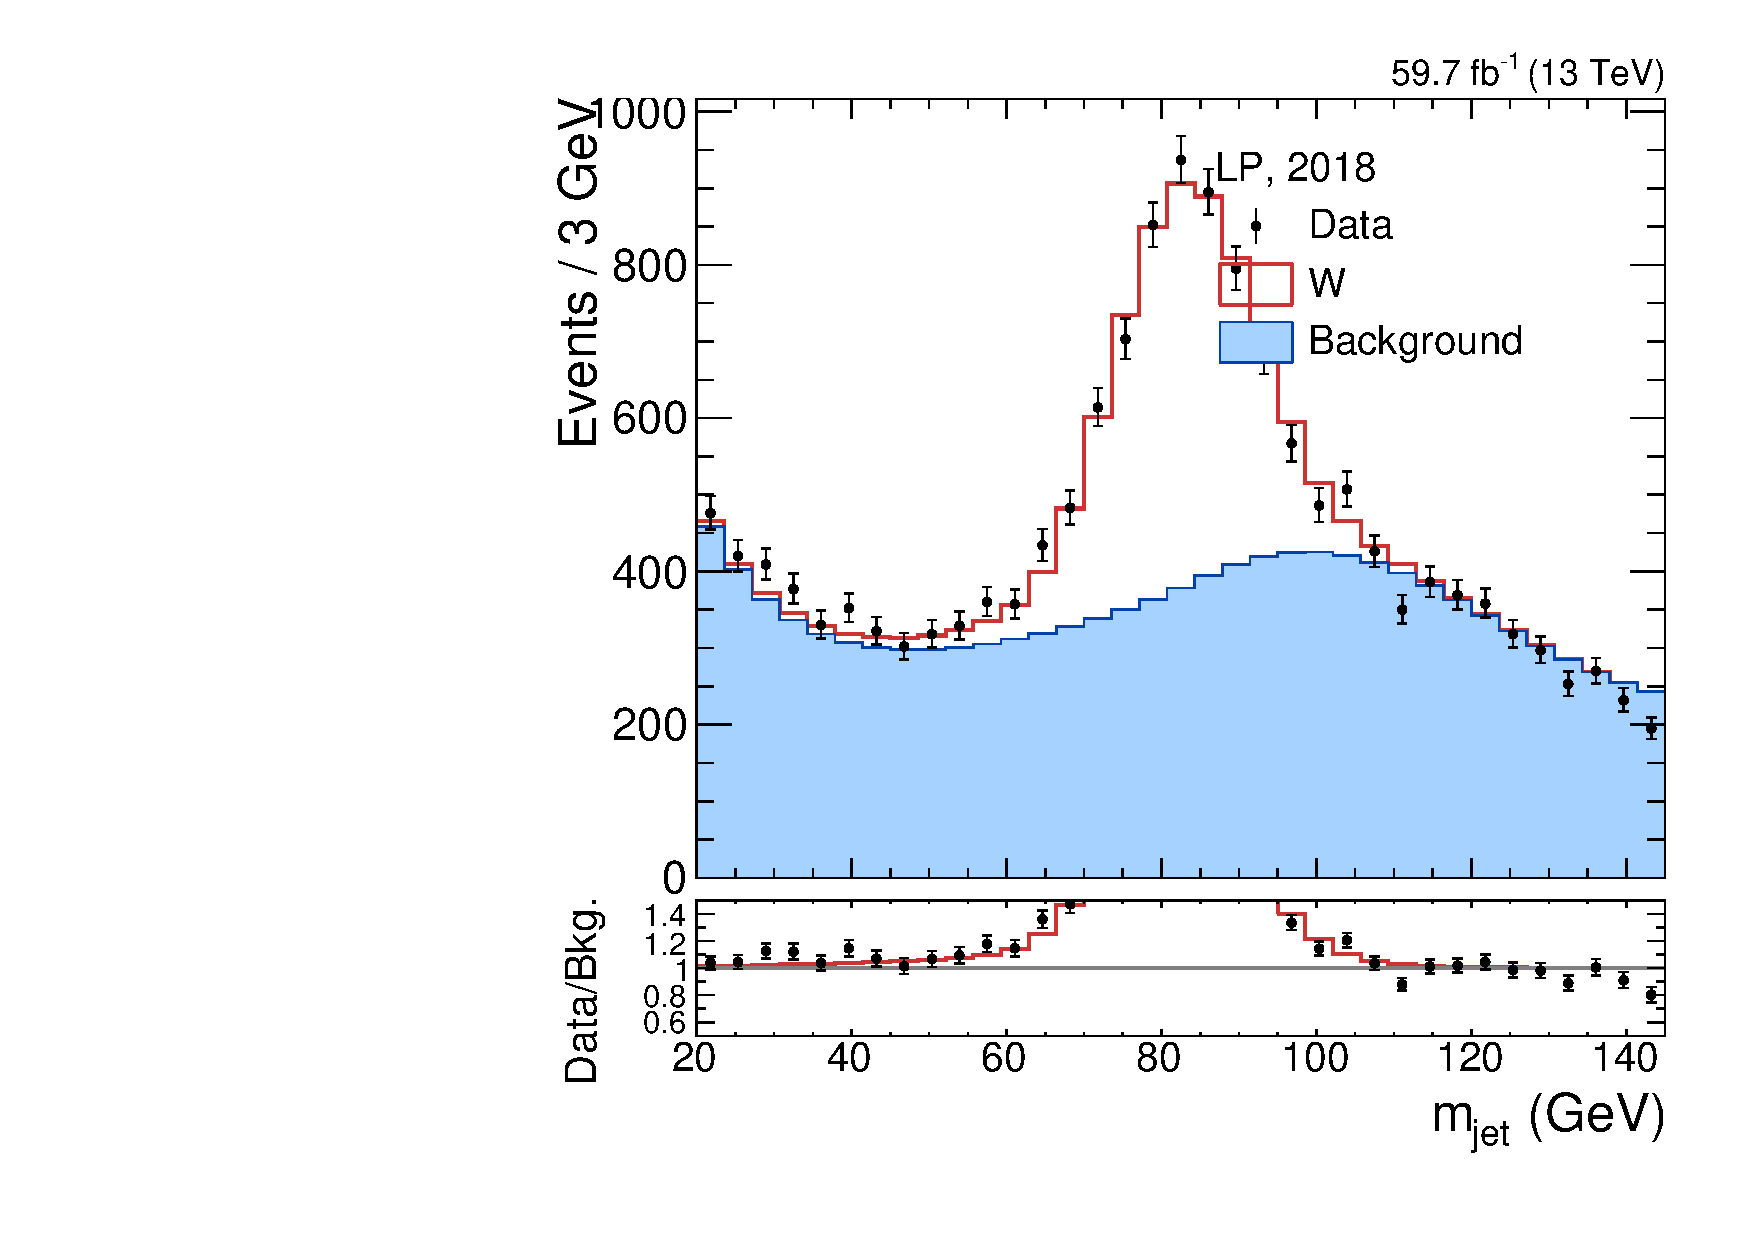
\includegraphics[width=0.3\textwidth]{fig/Vtag/PostFit__MJJ__allC_allL_LP_2018.pdf}
  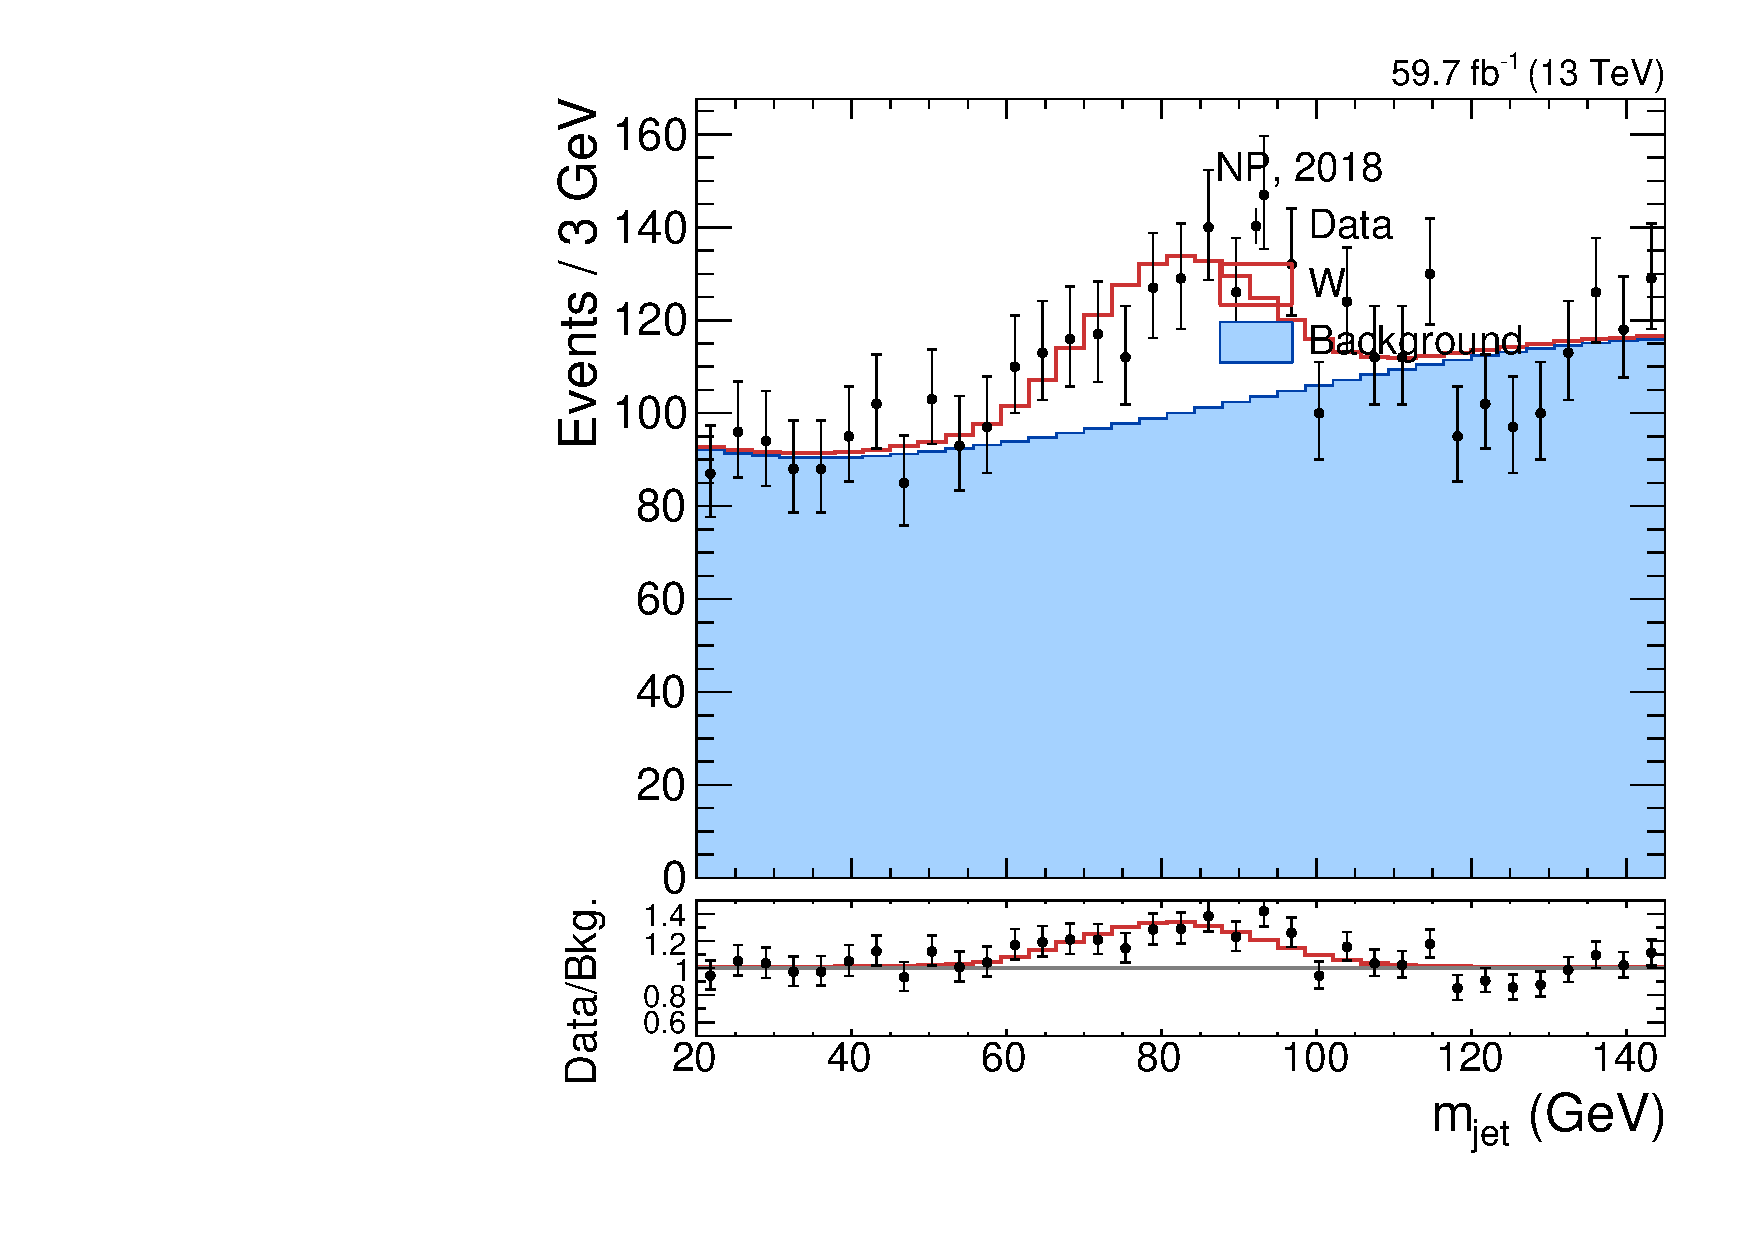
\includegraphics[width=0.3\textwidth]{fig/Vtag/PostFit__MJJ__allC_allL_NP_2018.pdf}\\
  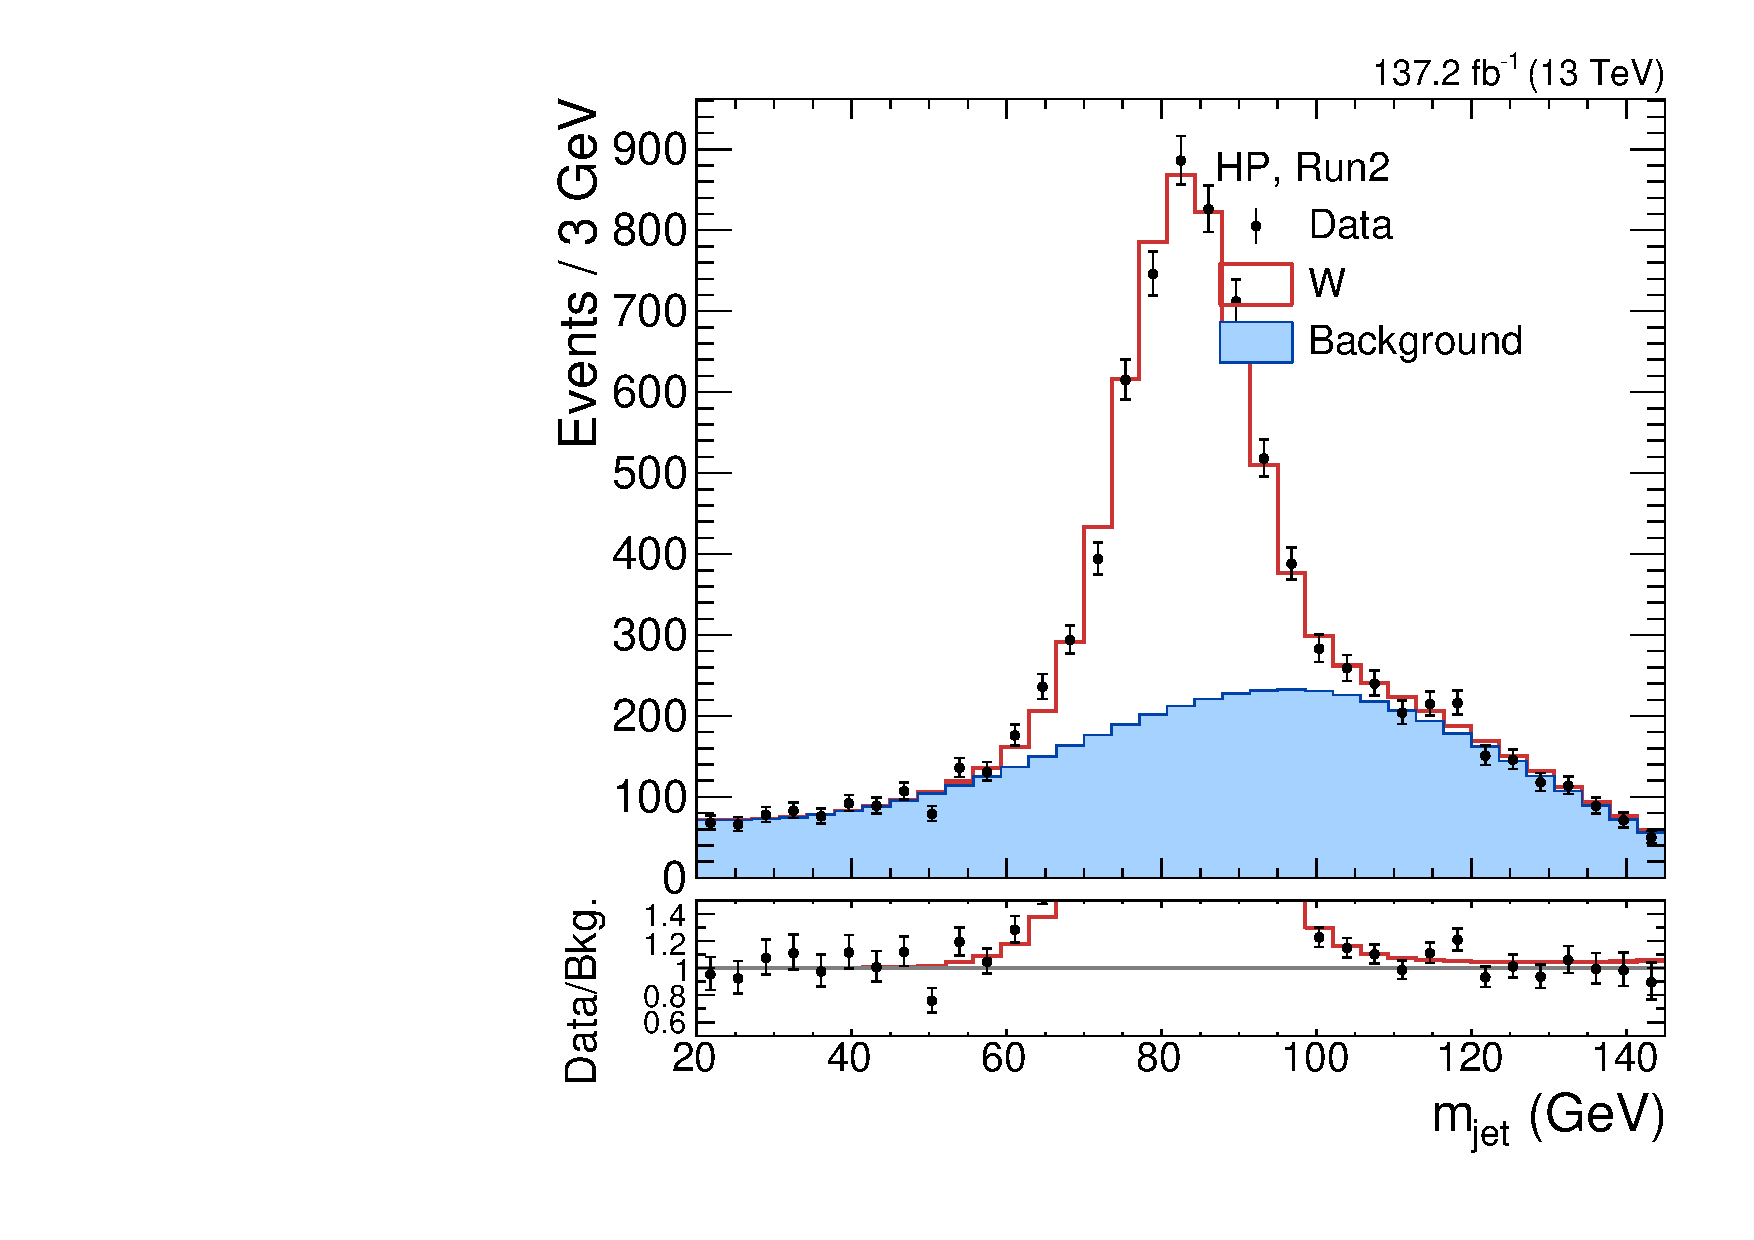
\includegraphics[width=0.3\textwidth]{fig/Vtag/PostFit__MJJ__allC_allL_HP_Run2.pdf}
  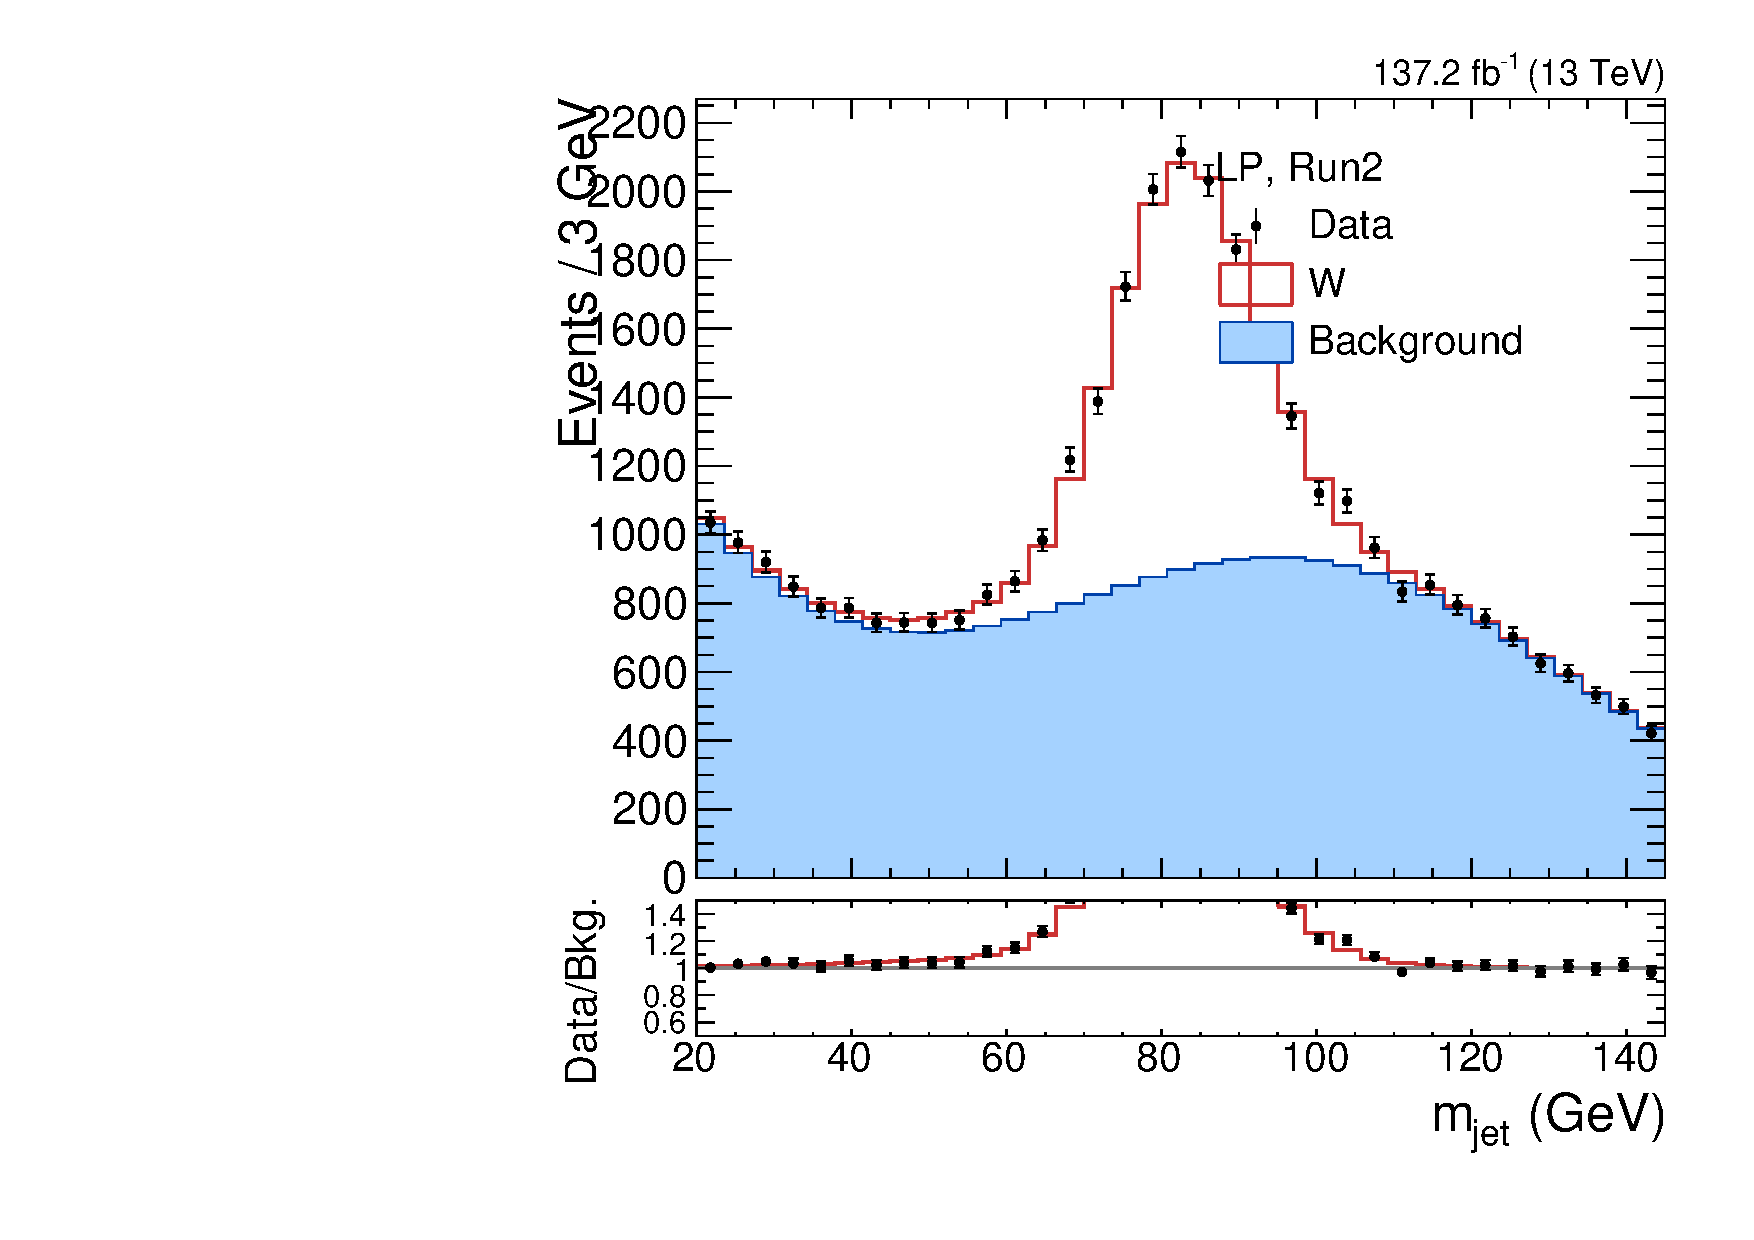
\includegraphics[width=0.3\textwidth]{fig/Vtag/PostFit__MJJ__allC_allL_LP_Run2.pdf}
  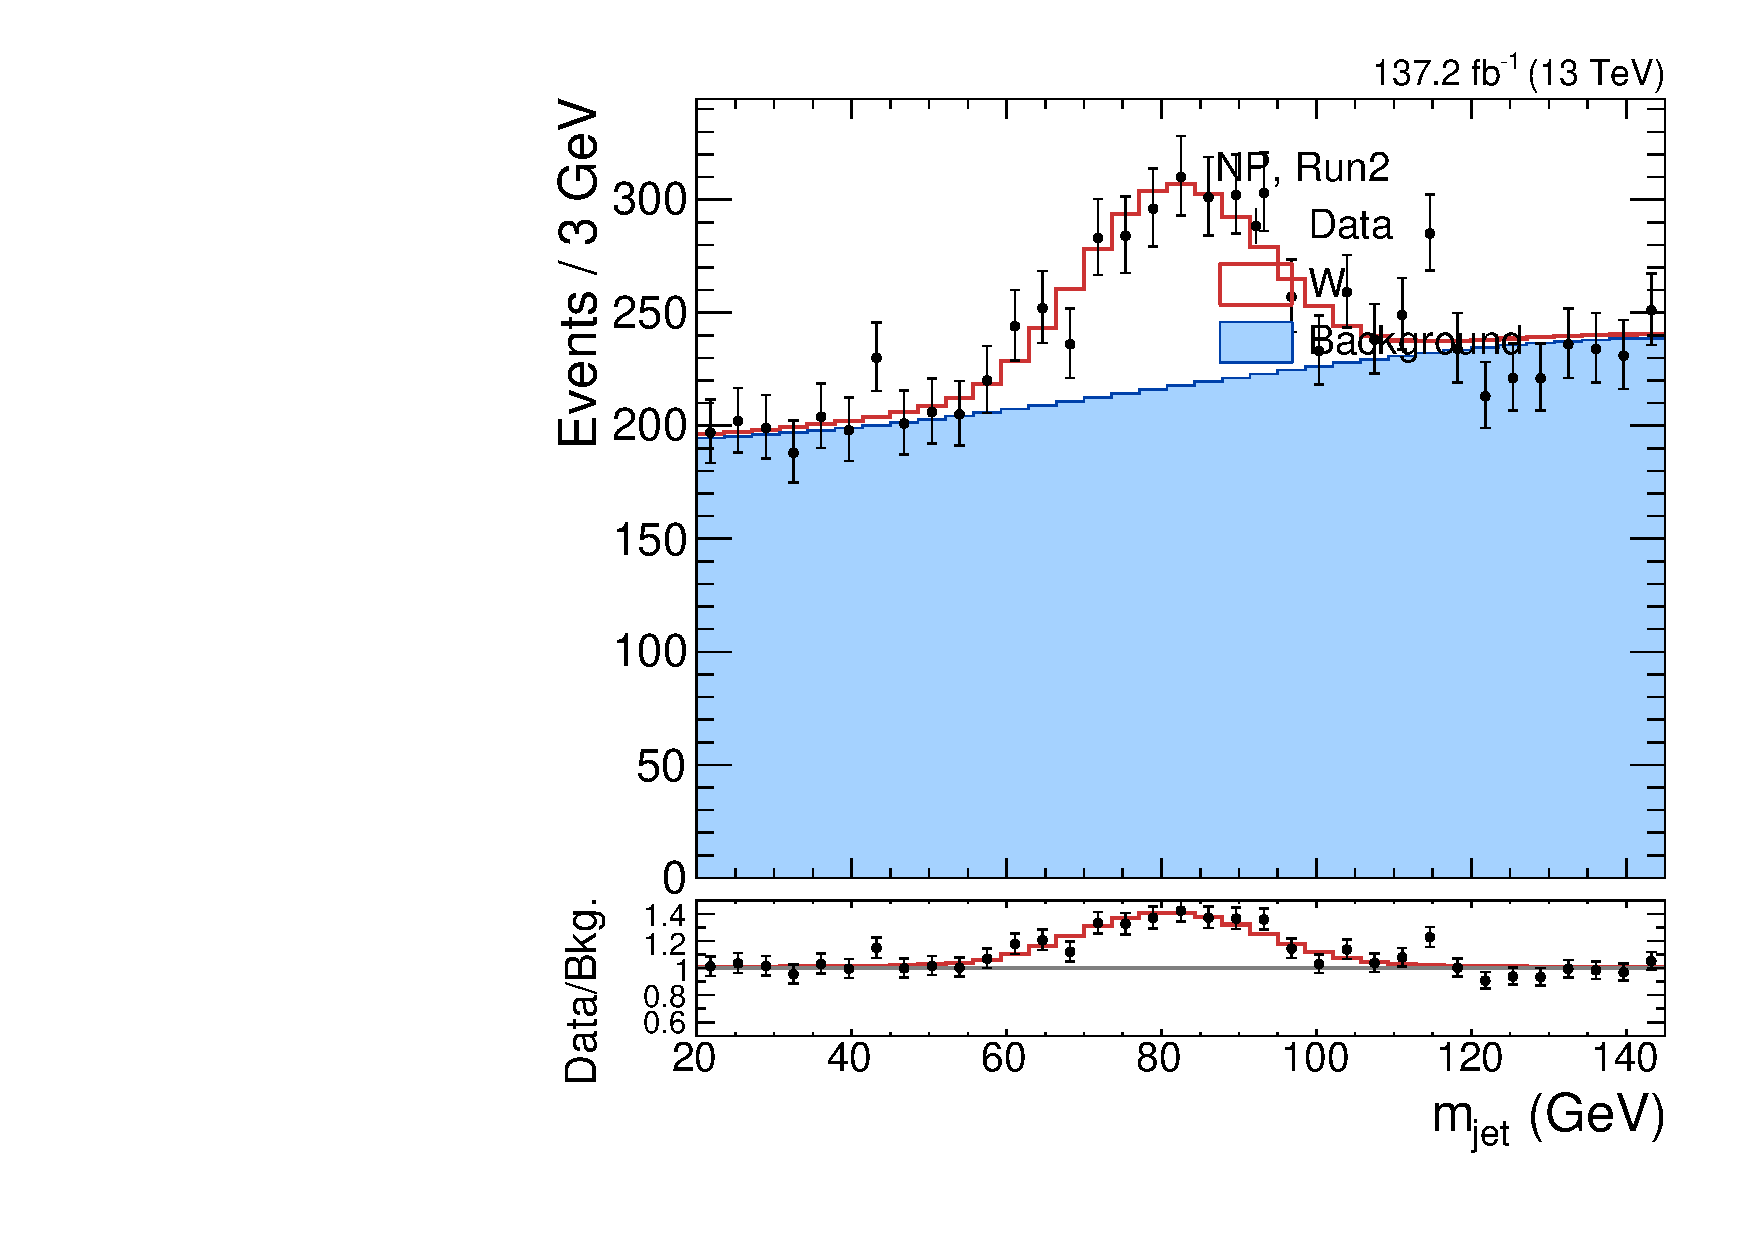
\includegraphics[width=0.3\textwidth]{fig/Vtag/PostFit__MJJ__allC_allL_NP_Run2.pdf}\\
  \caption{
    Post-fit distributions for the background MC and dataset for all three years and Run 2 (from top to bottom: 2016, 2017, 2018, Run 2), and for the three purity categories (from left to right: HP, LP, NP).
  }
  \label{fig:VTag_postfit_Run2}
\end{figure}

\begin{table}[htbp]
  \centering
  % !TEX root = ../../thesis.tex
\footnotesize
\begin{tabular}{|ccc|}
  \hline
  Year & HP & LP \\
  \hline
  2016  & $1.02 \pm 0.04$ (stat) $\pm 0.03$ (syst) & $0.98 \pm 0.02$ (stat) $\pm 0.03$ (syst)  \\
  2017  & $0.83 \pm 0.04$ (stat) $\pm 0.03$ (syst) & $1.10 \pm 0.02$ (stat) $\pm 0.03$ (syst)  \\
  2018  & $0.87 \pm 0.03$ (stat) $\pm 0.03$ (syst) & $1.08 \pm 0.02$ (stat) $\pm 0.03$ (syst)  \\
  Run 2 & $0.88 \pm 0.02$ (stat) $\pm 0.03$ (syst) & $1.06 \pm 0.02$ (stat) $\pm 0.03$ (syst)  \\
  \hline
\end{tabular}

  \caption{
    $V$-tagging scale factors for the HP and LP categories obtained from the fit process.
  }
  \label{tab:VTagFactors}
\end{table}

\begin{table}[htbp]
  \centering
  % !TEX root = ../../thesis.tex
\footnotesize
\begin{tabular}{c|c|c}
  \hline
  Year & Scale & Resolution \\
  \hline
  \hline
  2016  & $0.991 \pm 0.003$ (stat) $\pm 0.002$ (syst) & $1.00 \pm 0.03$ (stat) $\pm 0.02$ (syst) \\
  2017  & $0.989 \pm 0.003$ (stat) $\pm 0.002$ (syst) & $1.07 \pm 0.04$ (stat) $\pm 0.02$ (syst) \\
  2018  & $0.987 \pm 0.002$ (stat) $\pm 0.002$ (syst) & $1.08 \pm 0.03$ (stat) $\pm 0.02$ (syst) \\
  Run 2 & $0.990 \pm 0.002$ (stat) $\pm 0.002$ (syst) & $1.08 \pm 0.02$ (stat) $\pm 0.02$ (syst) \\
  \hline
\end{tabular}

  \caption{
    Scale factors for the jet mass scale and resolution obtained from the fit process.
  }
  \label{tab:VScaleRes}
\end{table}

\subsection{Momentum Dependence}

% Momentum dependence
We also conduct a study on the dependence of the $V$-tagging scale factors as a function of the diboson invariant mass \MVV to apply a systematic uncertainty on the $V$-tagging process.
To do so, we measure the $V$-tagging scale factors for the full Run 2 dataset, but in three different binnings of \MVV.
We apply a low-mass binning of $[0.6,0.8\unit{TeV}]$, a mid-mass binning of $[0.8,1.0\unit{TeV}]$, and a high-mass binning of $[1.0,1.5\unit{TeV}]$.
The resulting post-fit distributions for all three binnings and for all purity categories may be see in figure~\ref{fig:VTag_postfit_massdep}.

\begin{figure}[htbp]
  \centering
  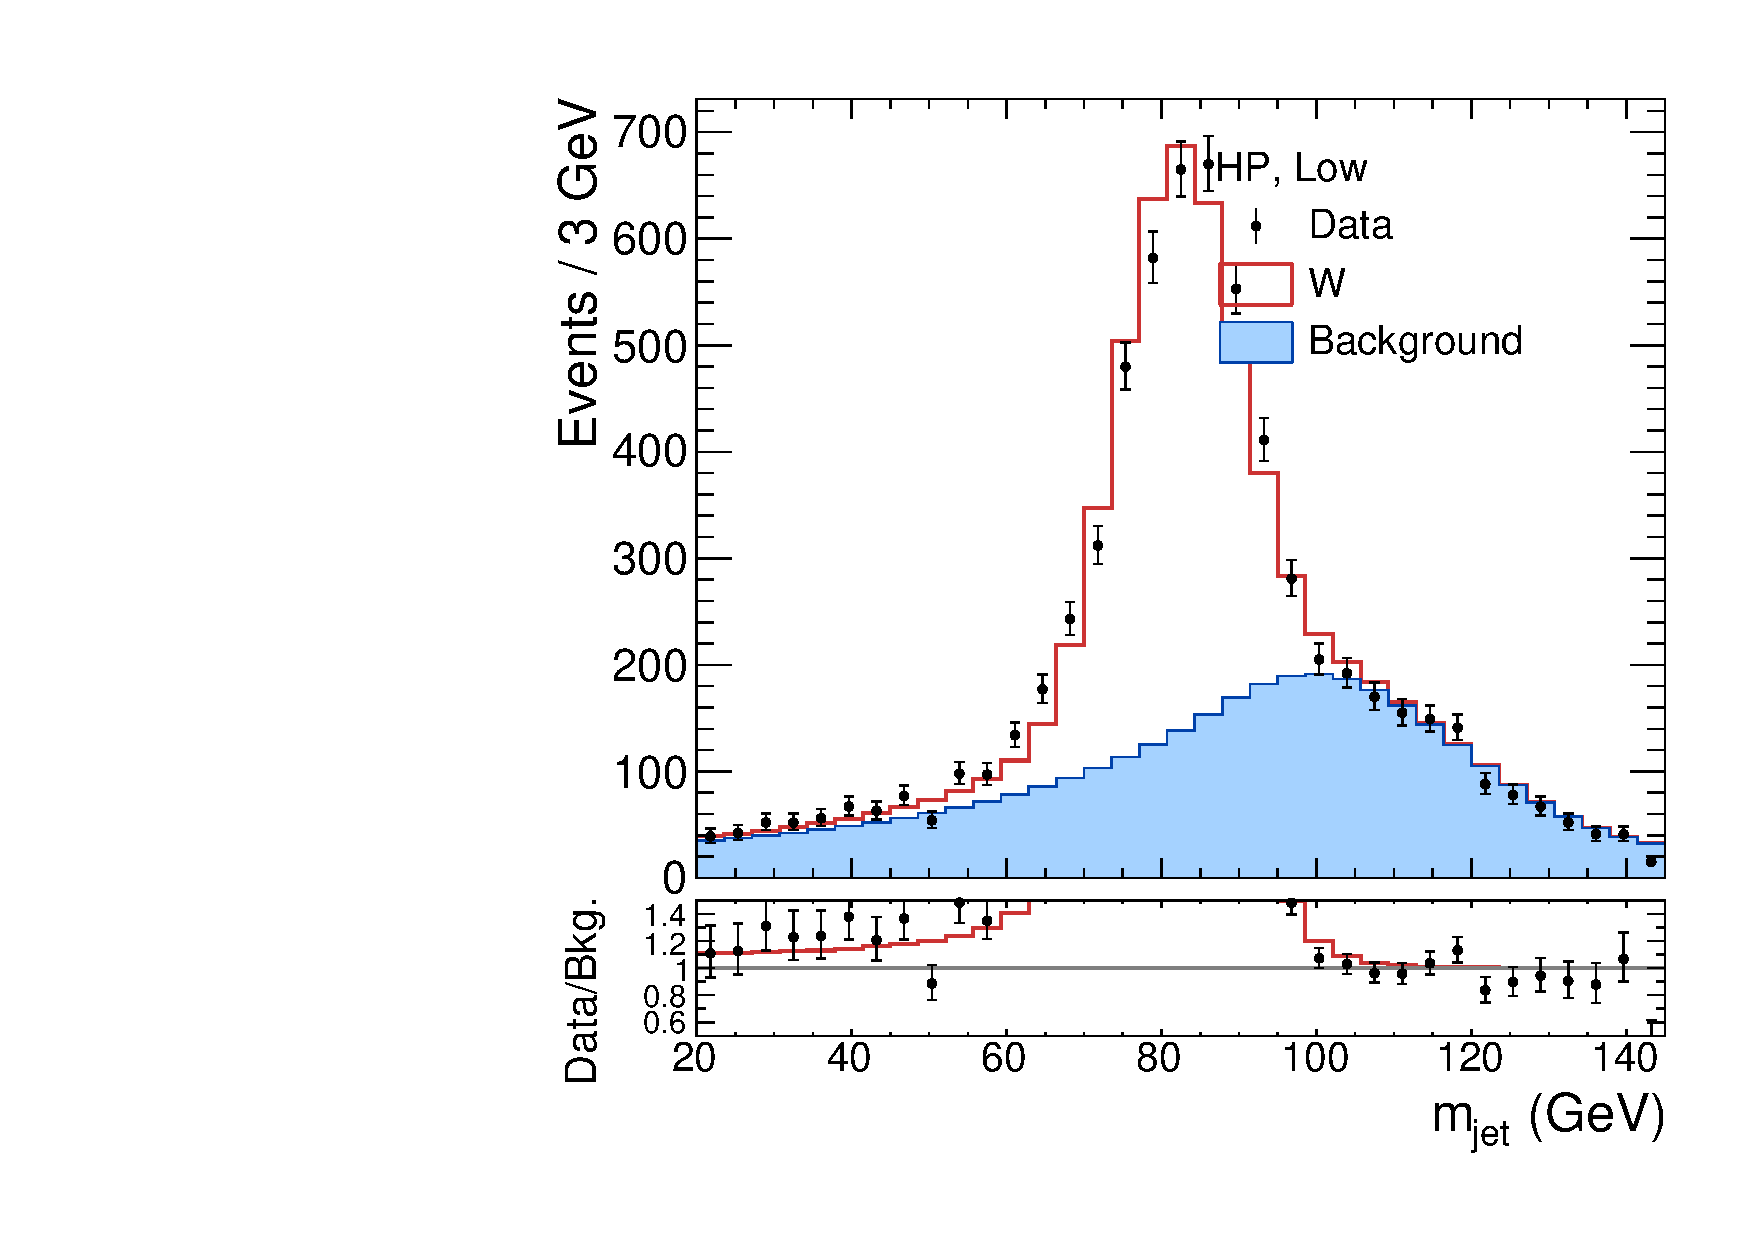
\includegraphics[width=0.3\textwidth]{fig/Vtag/PostFit__MJJ__allC_allL_HP_Low.pdf}
  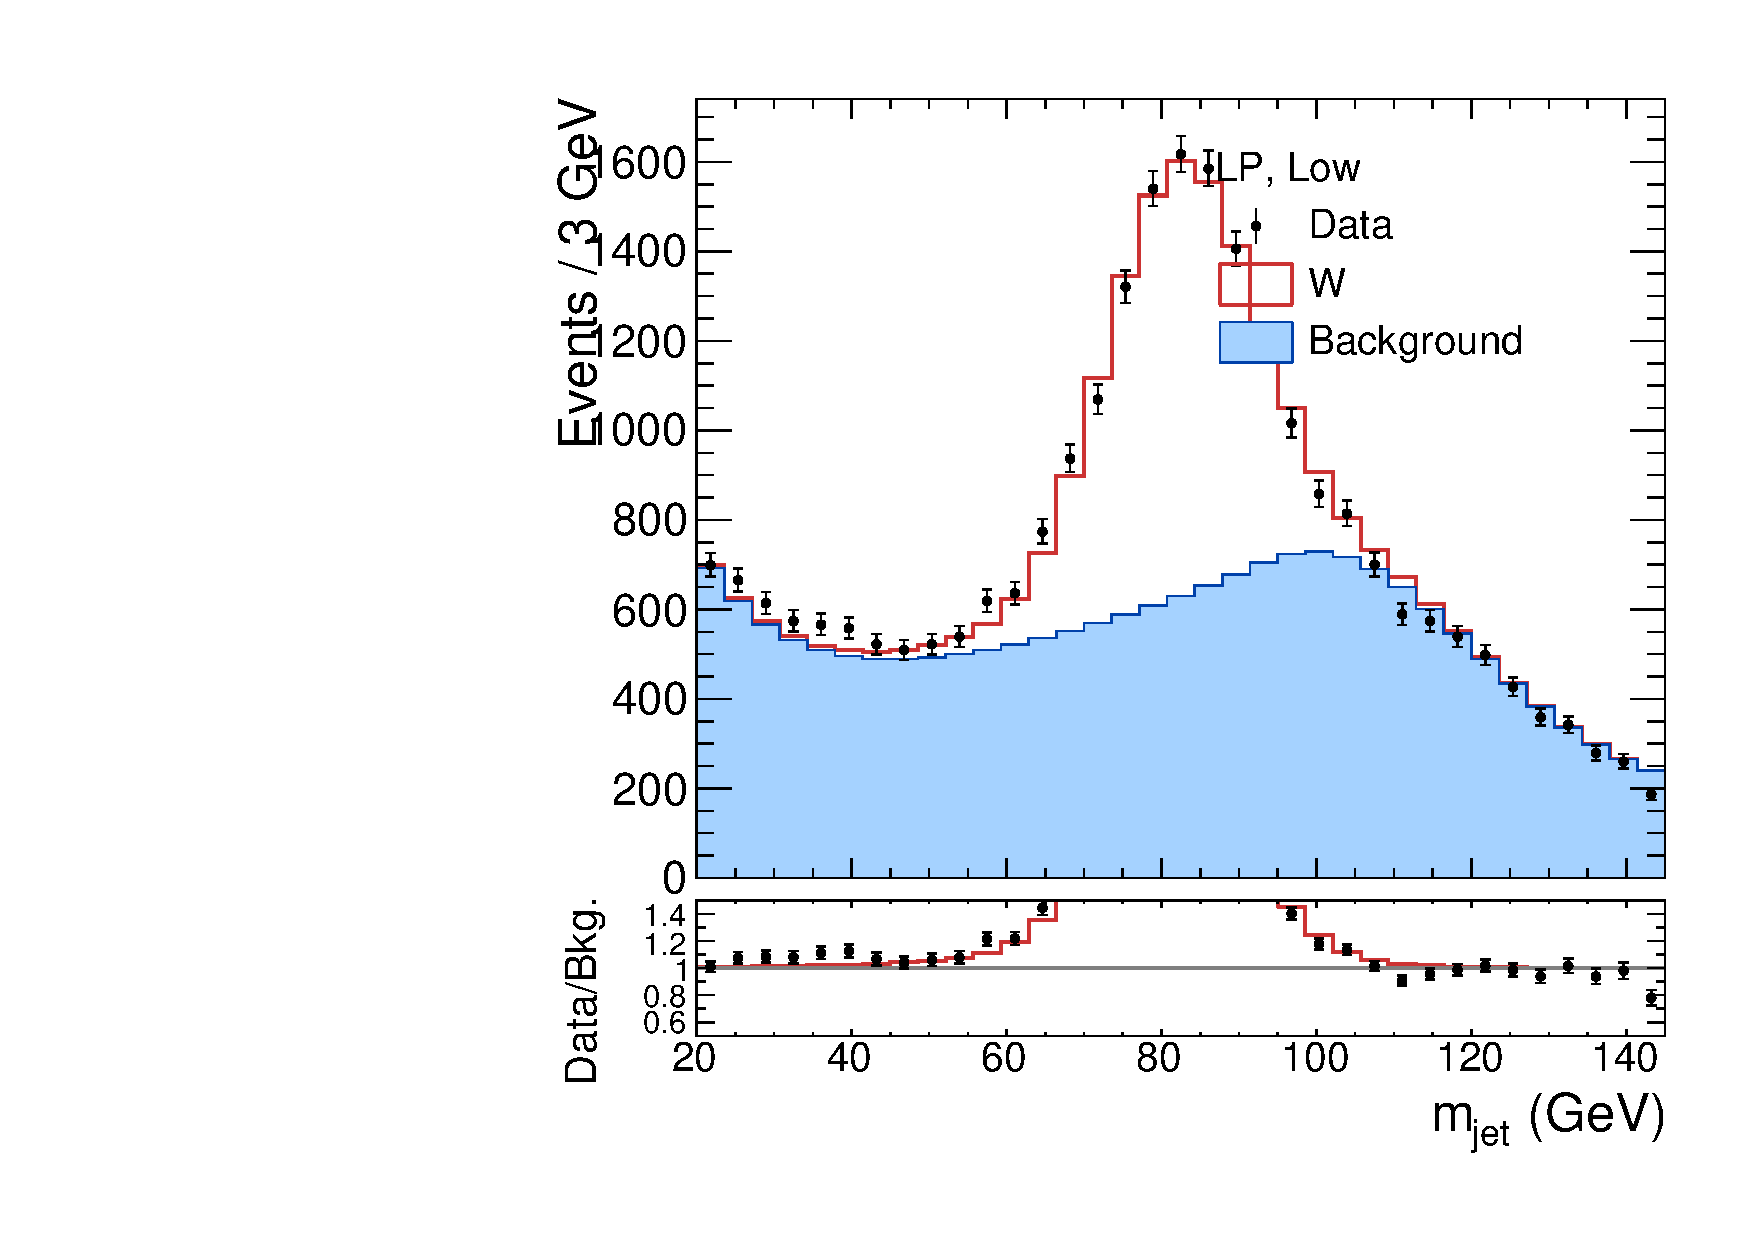
\includegraphics[width=0.3\textwidth]{fig/Vtag/PostFit__MJJ__allC_allL_LP_Low.pdf}
  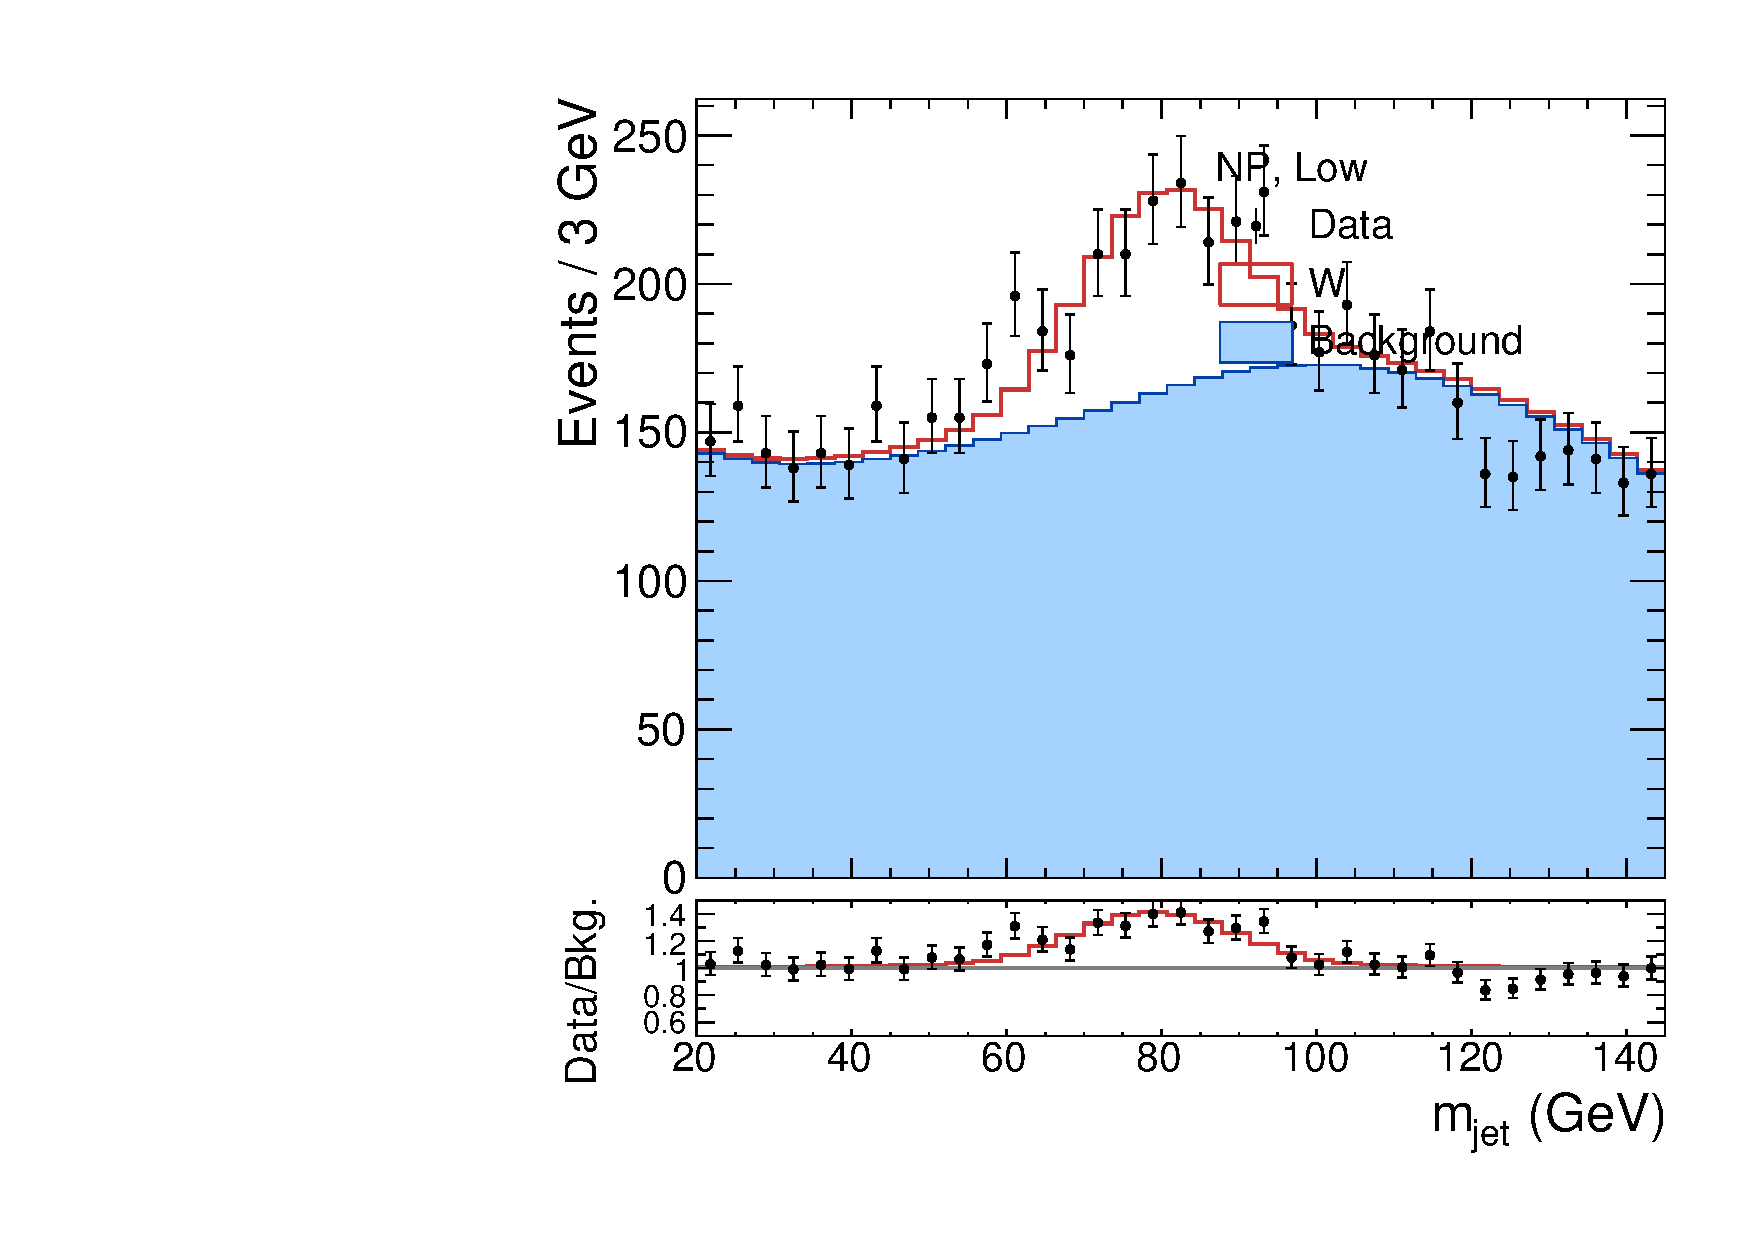
\includegraphics[width=0.3\textwidth]{fig/Vtag/PostFit__MJJ__allC_allL_NP_Low.pdf}\\
  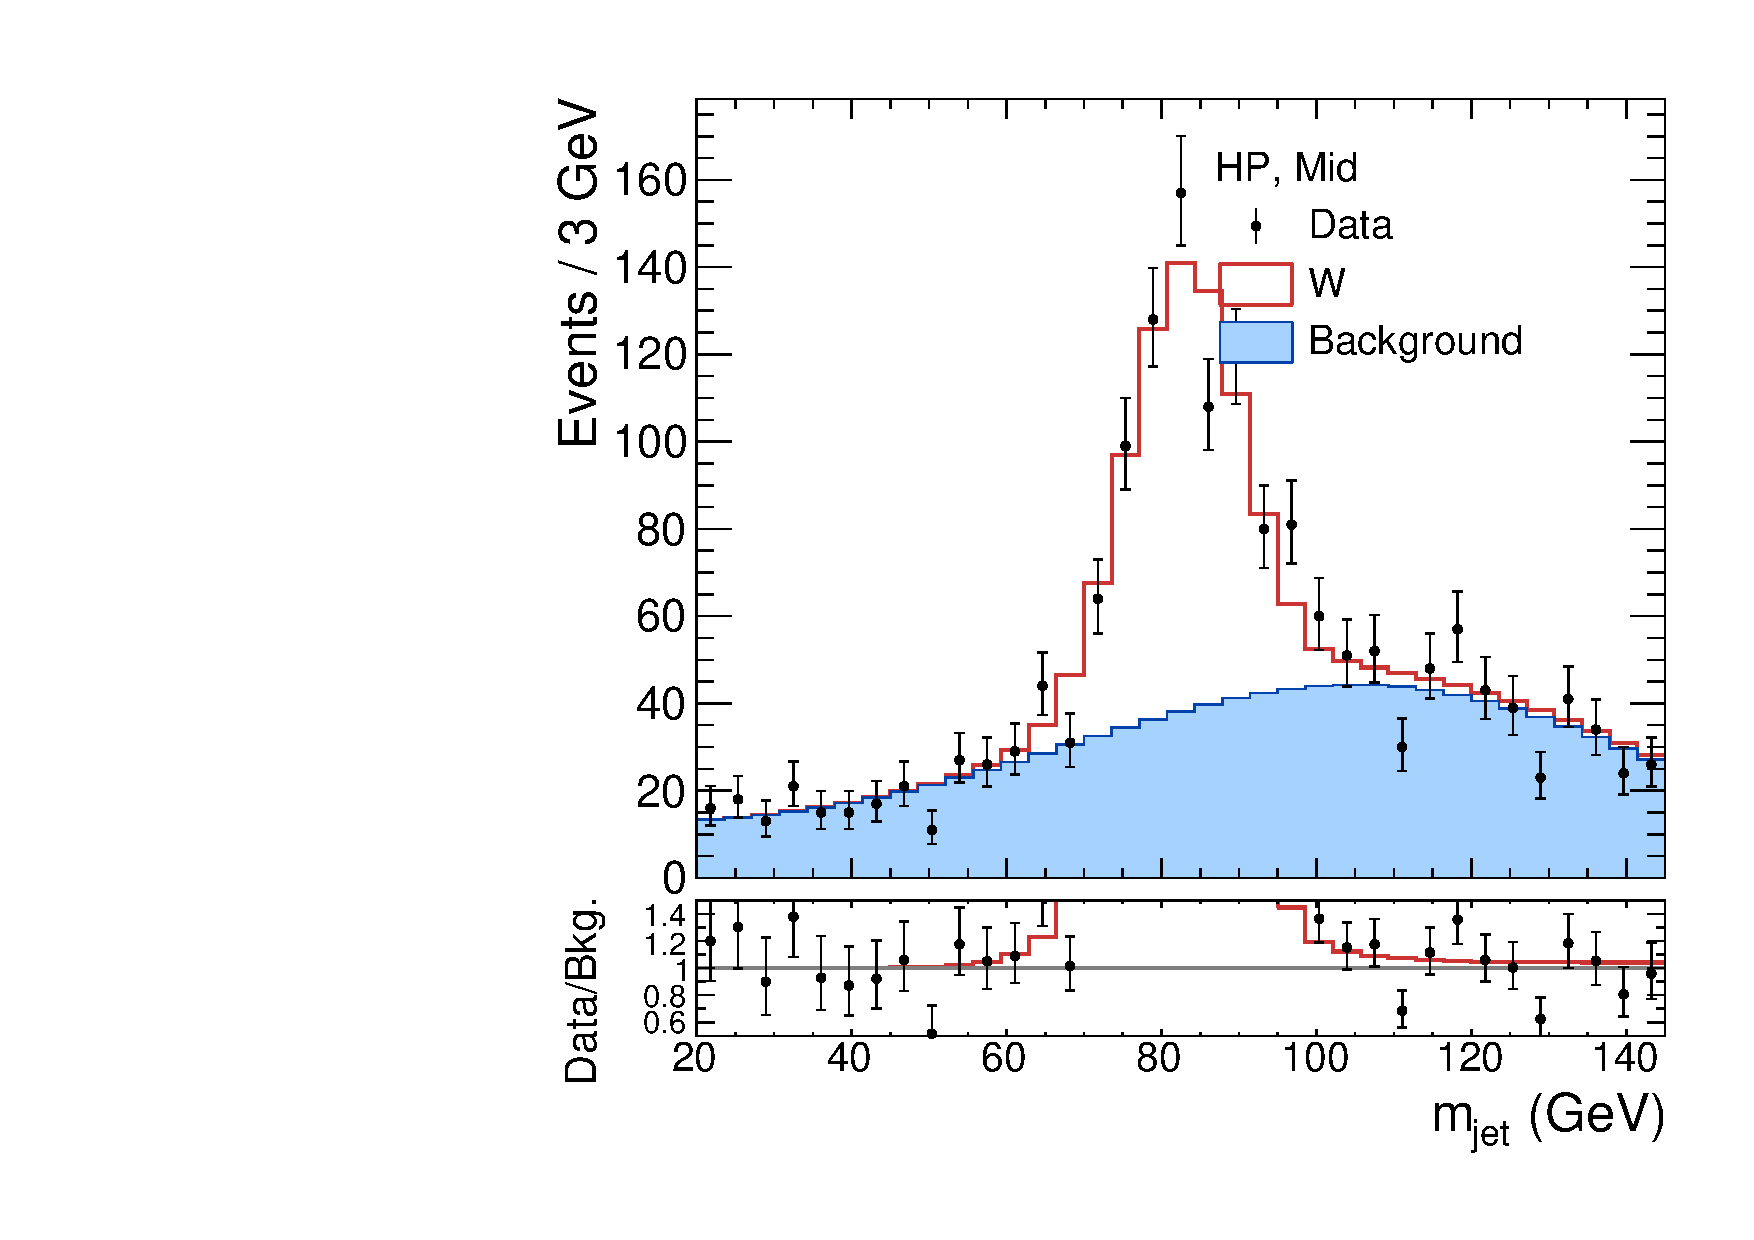
\includegraphics[width=0.3\textwidth]{fig/Vtag/PostFit__MJJ__allC_allL_HP_Mid.pdf}
  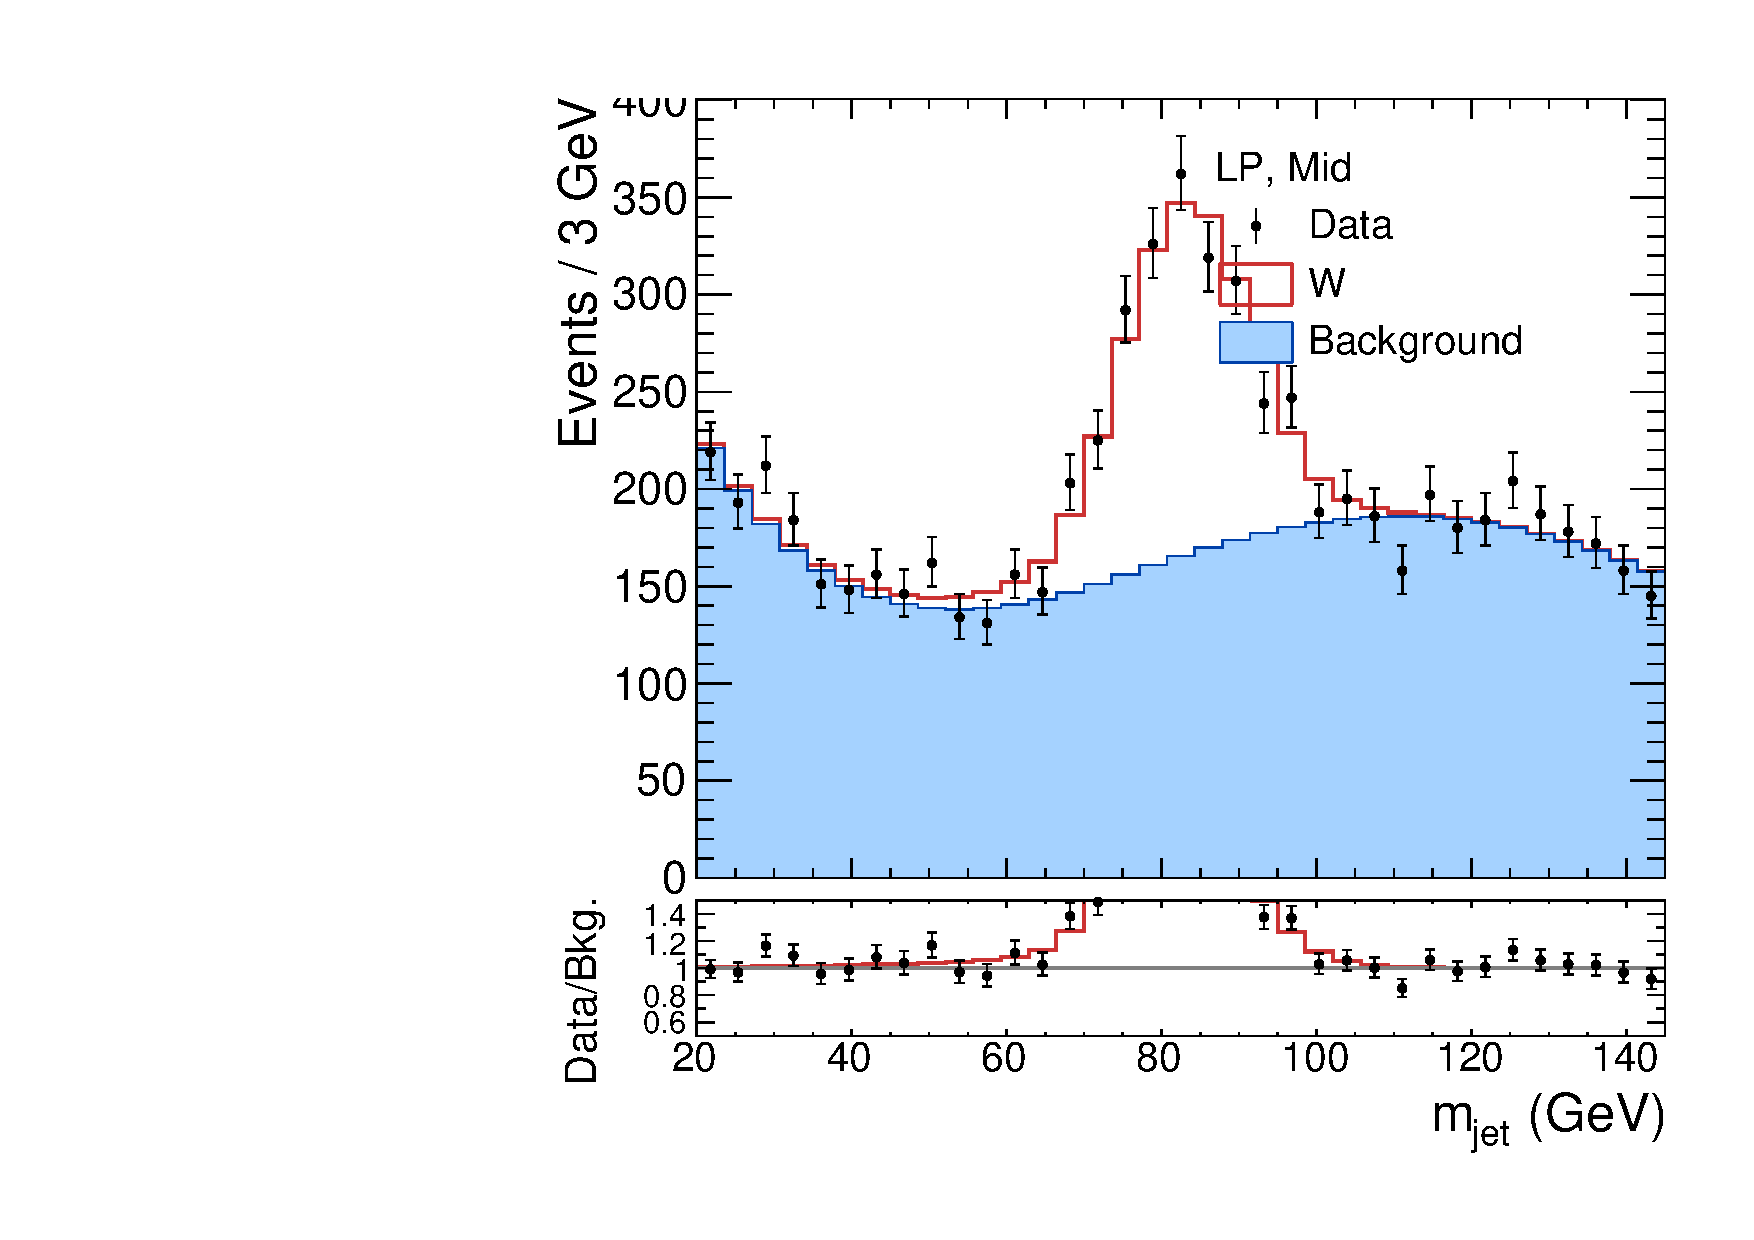
\includegraphics[width=0.3\textwidth]{fig/Vtag/PostFit__MJJ__allC_allL_LP_Mid.pdf}
  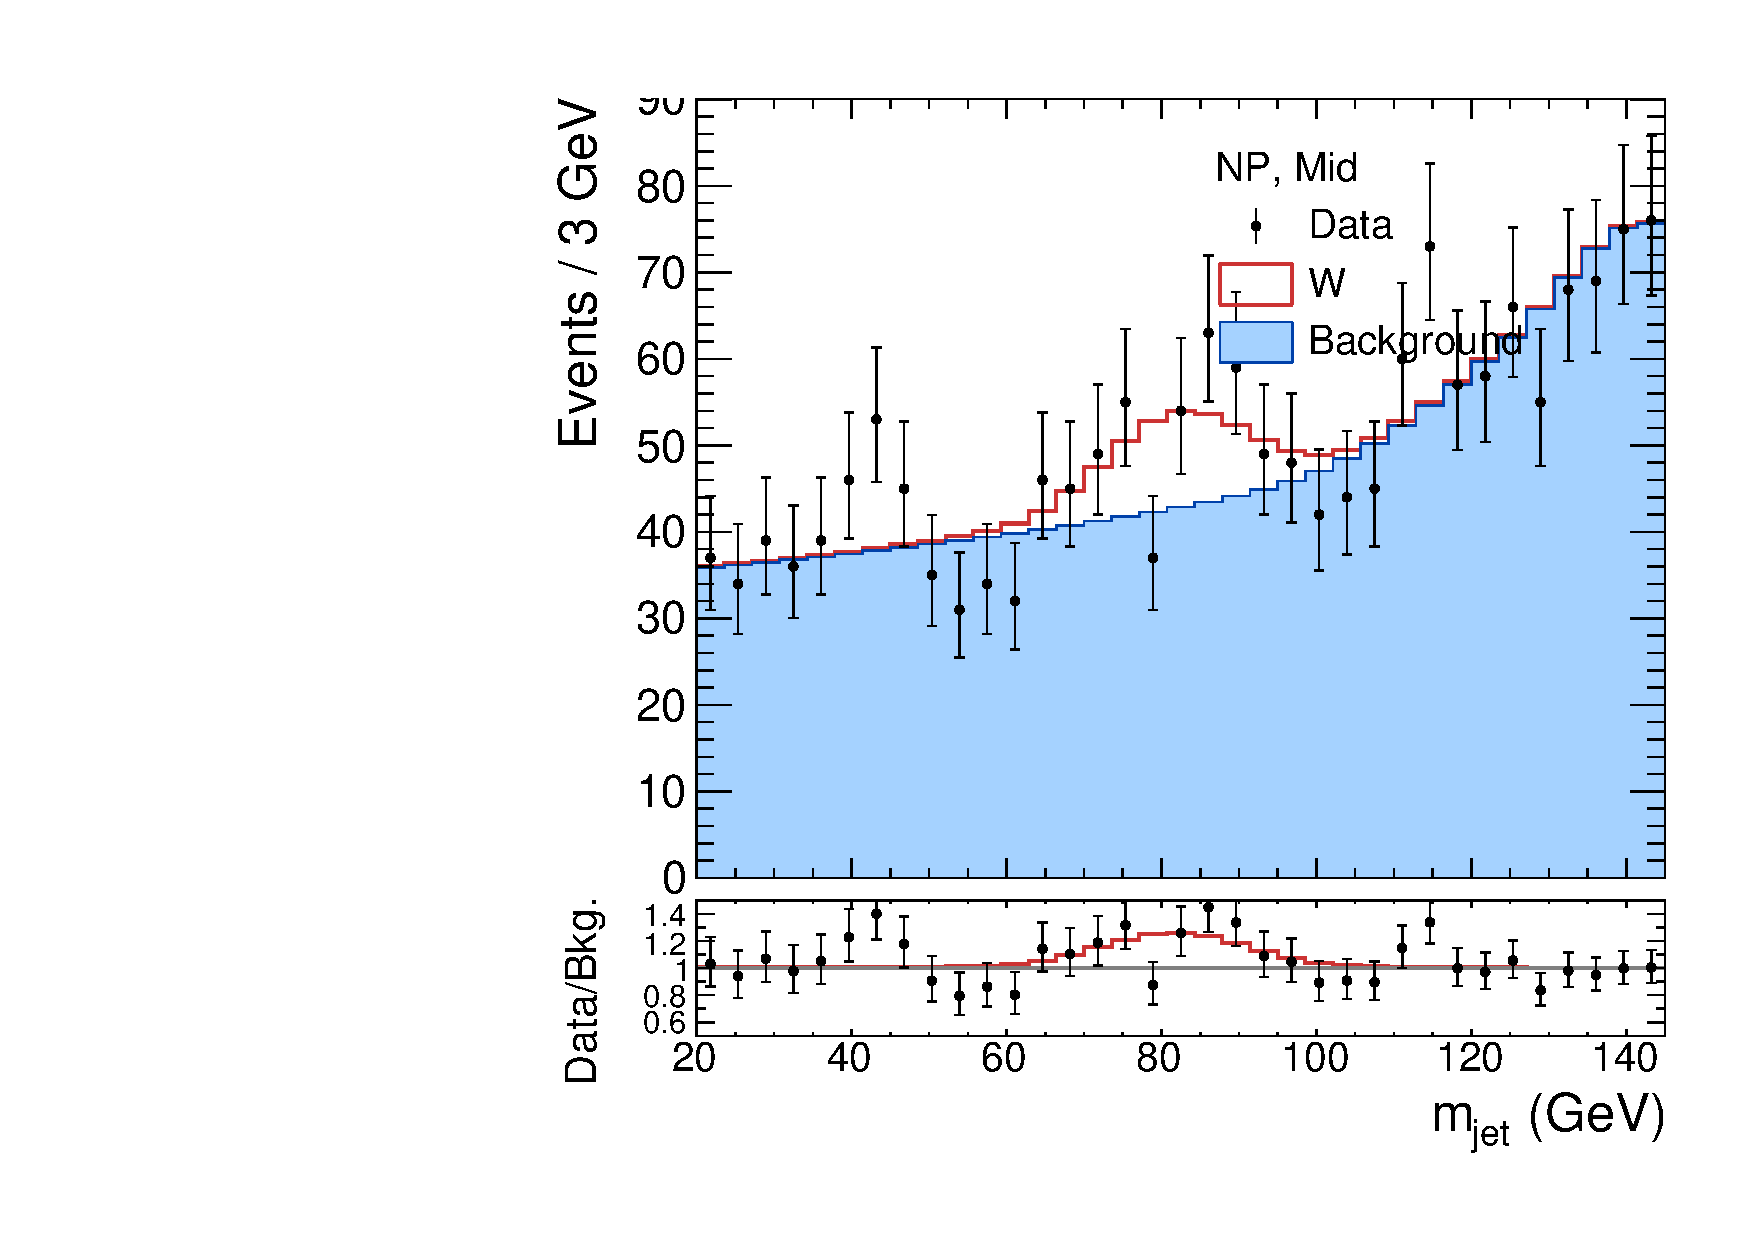
\includegraphics[width=0.3\textwidth]{fig/Vtag/PostFit__MJJ__allC_allL_NP_Mid.pdf}\\
  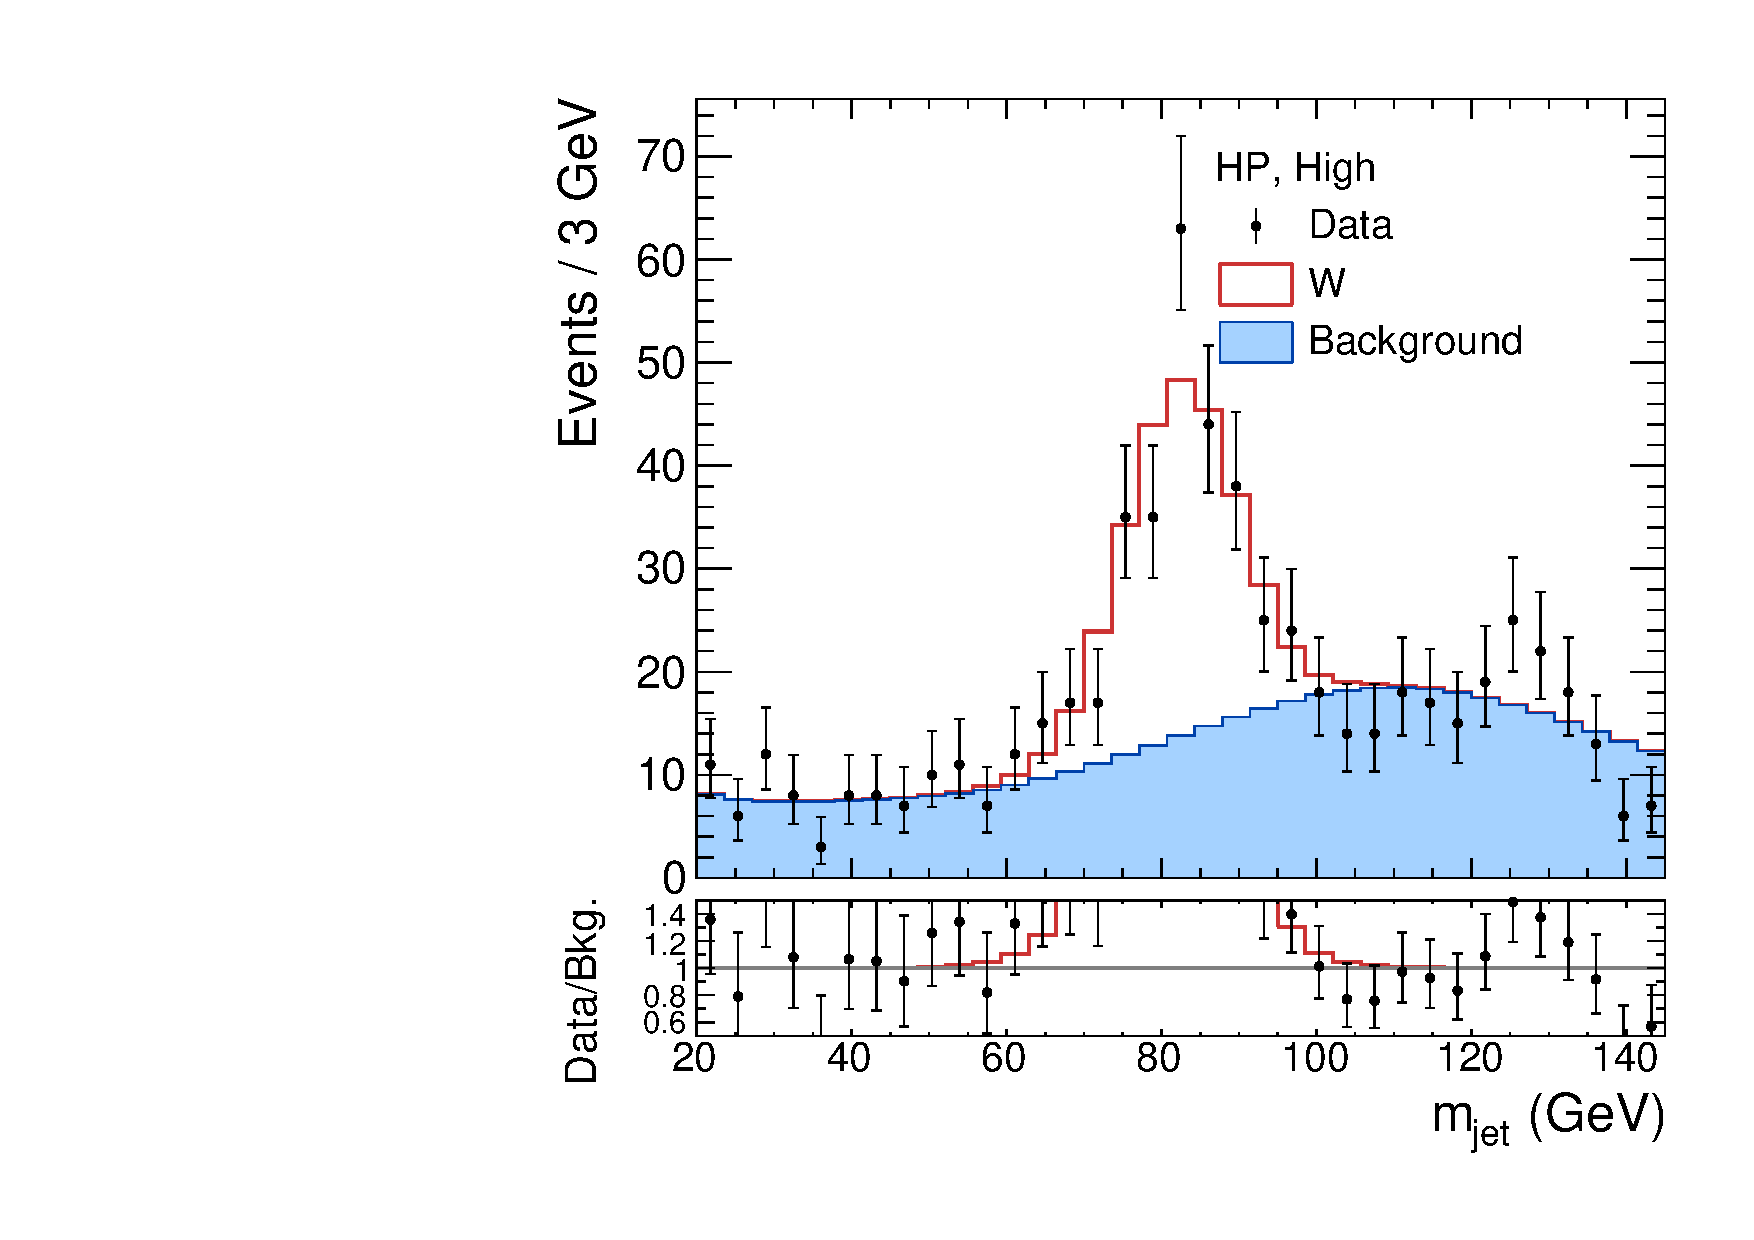
\includegraphics[width=0.3\textwidth]{fig/Vtag/PostFit__MJJ__allC_allL_HP_High.pdf}
  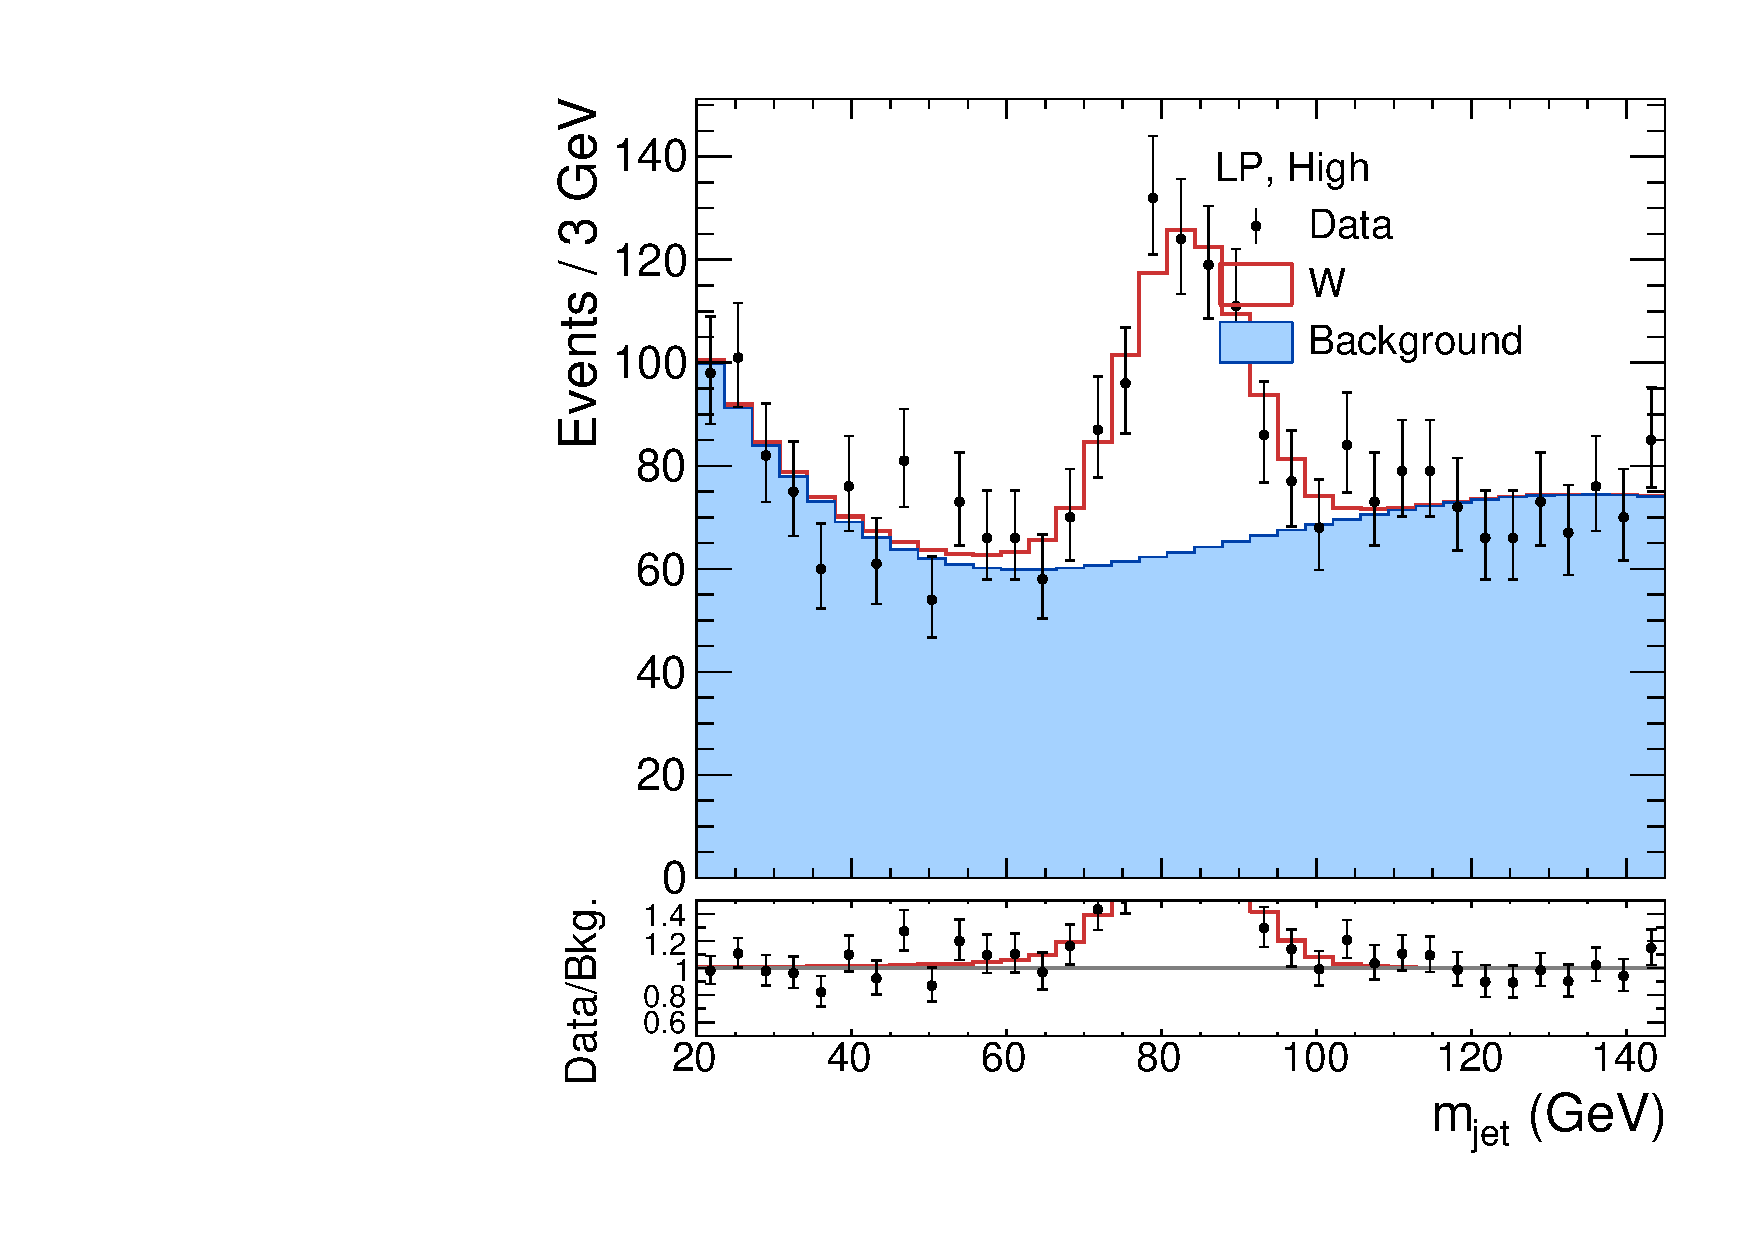
\includegraphics[width=0.3\textwidth]{fig/Vtag/PostFit__MJJ__allC_allL_LP_High.pdf}
  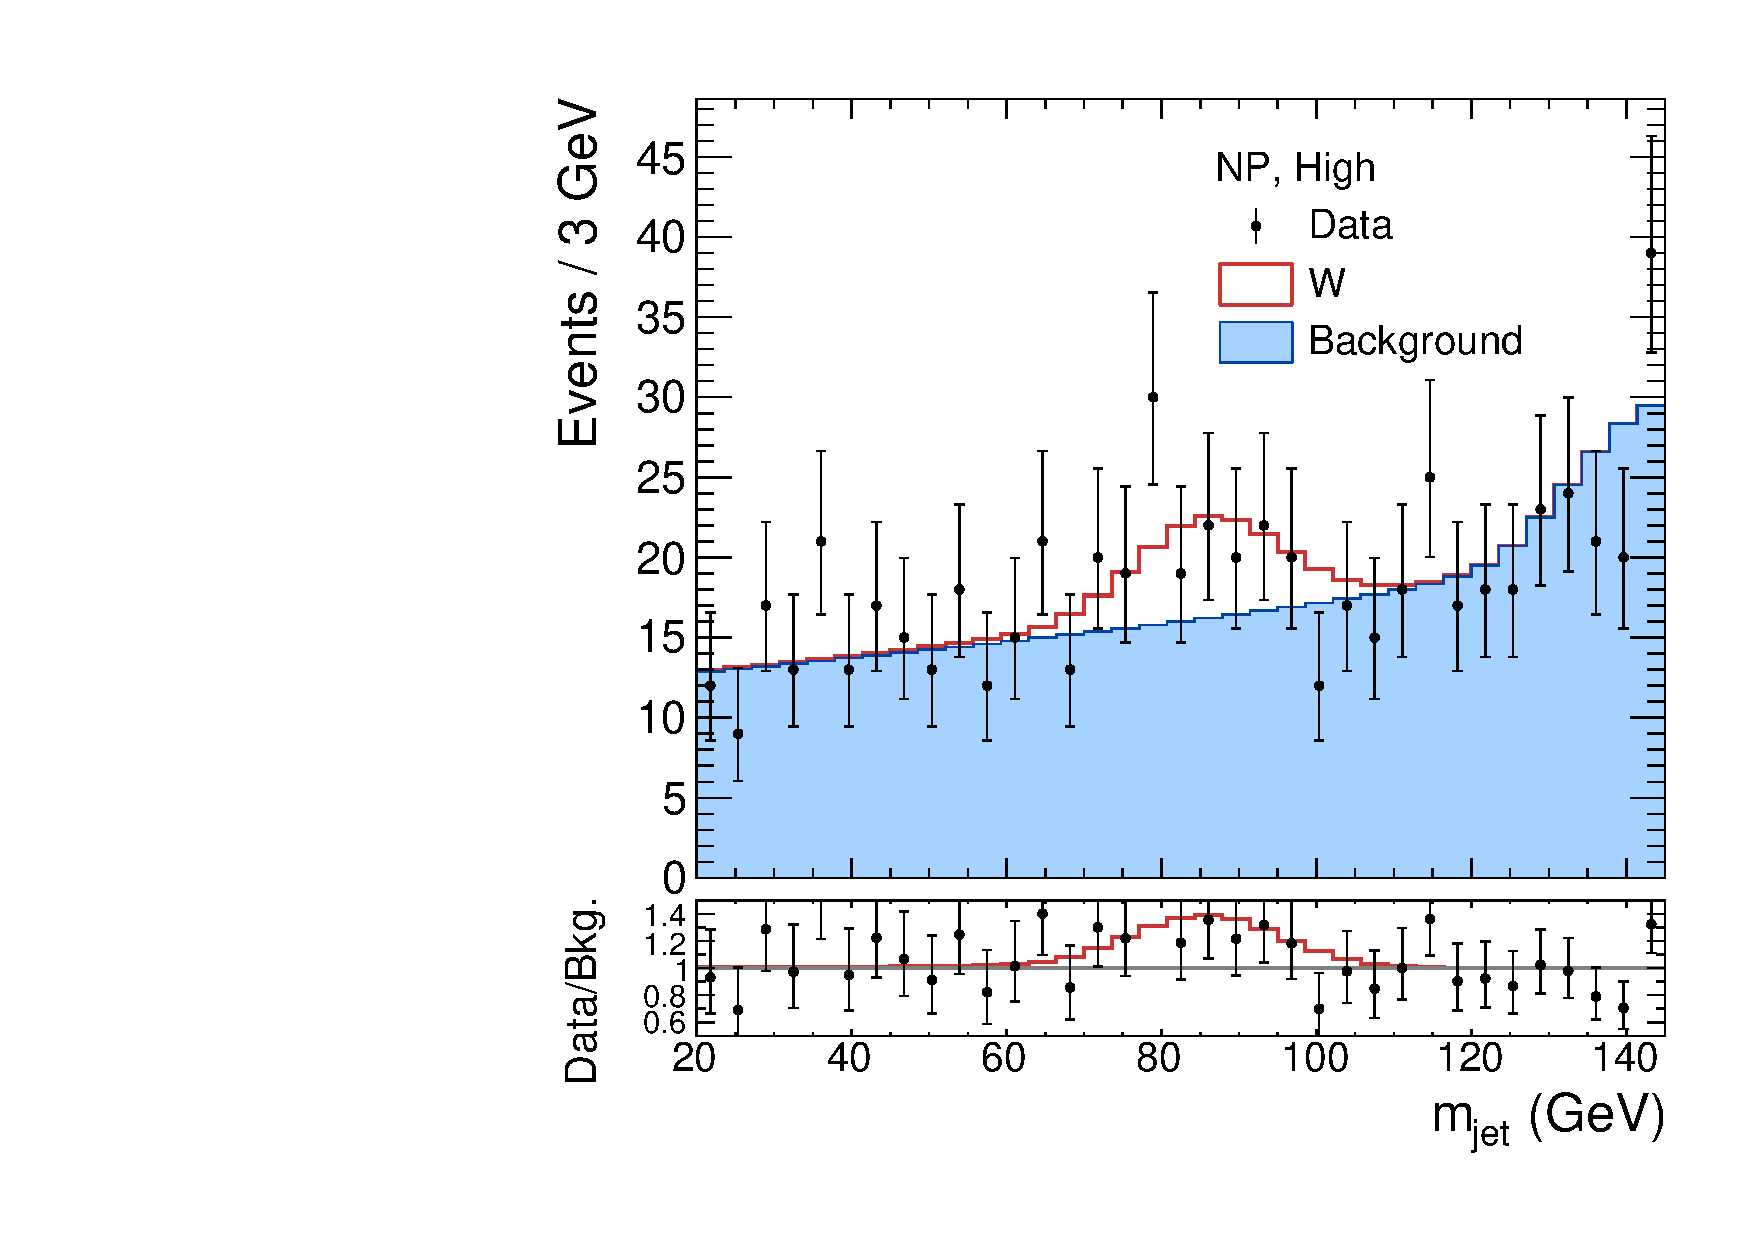
\includegraphics[width=0.3\textwidth]{fig/Vtag/PostFit__MJJ__allC_allL_NP_High.pdf}\\
  \caption{
    Post-fit distributions for three bins of the diboson invariant mass \MVV (from top to bottom: $[0.6,0.8\unit{TeV}]$, $[0.8,1.0\unit{TeV}]$, and $[1.0,1.5\unit{TeV}]$), in the three purity categories (from left to right: HP, LP, NP), for the full Run 2 dataset.
  }
  \label{fig:VTag_postfit_massdep}
\end{figure}

% Scale factors and efficiency
The resulting scale factors, scale, and resolution as a function of \MVV are plotted in figure~\ref{fig:VTag_massdep_summary} (left).
We observe no significant dependence for $V$-tagging as a function of \MVV for the three binnings used in this study.
The $V$-tagging efficiency as a function of \MVV is also studied, which can be seen in figure~\ref{fig:VTag_massdep_summary} (right).
This allows us to place an upper limit on the uncertainty of the \pt dependence.
The fact that the scale factor is small and the simulation agrees with the data means that the scale factor will never be larger than the variations of the efficiency versus \MVV. % May need to reword
At high mass, we may therefore set an uncertainty equal to the difference of the signal efficiency at high mass versus low mass.

\begin{figure}[htbp]
  \centering
  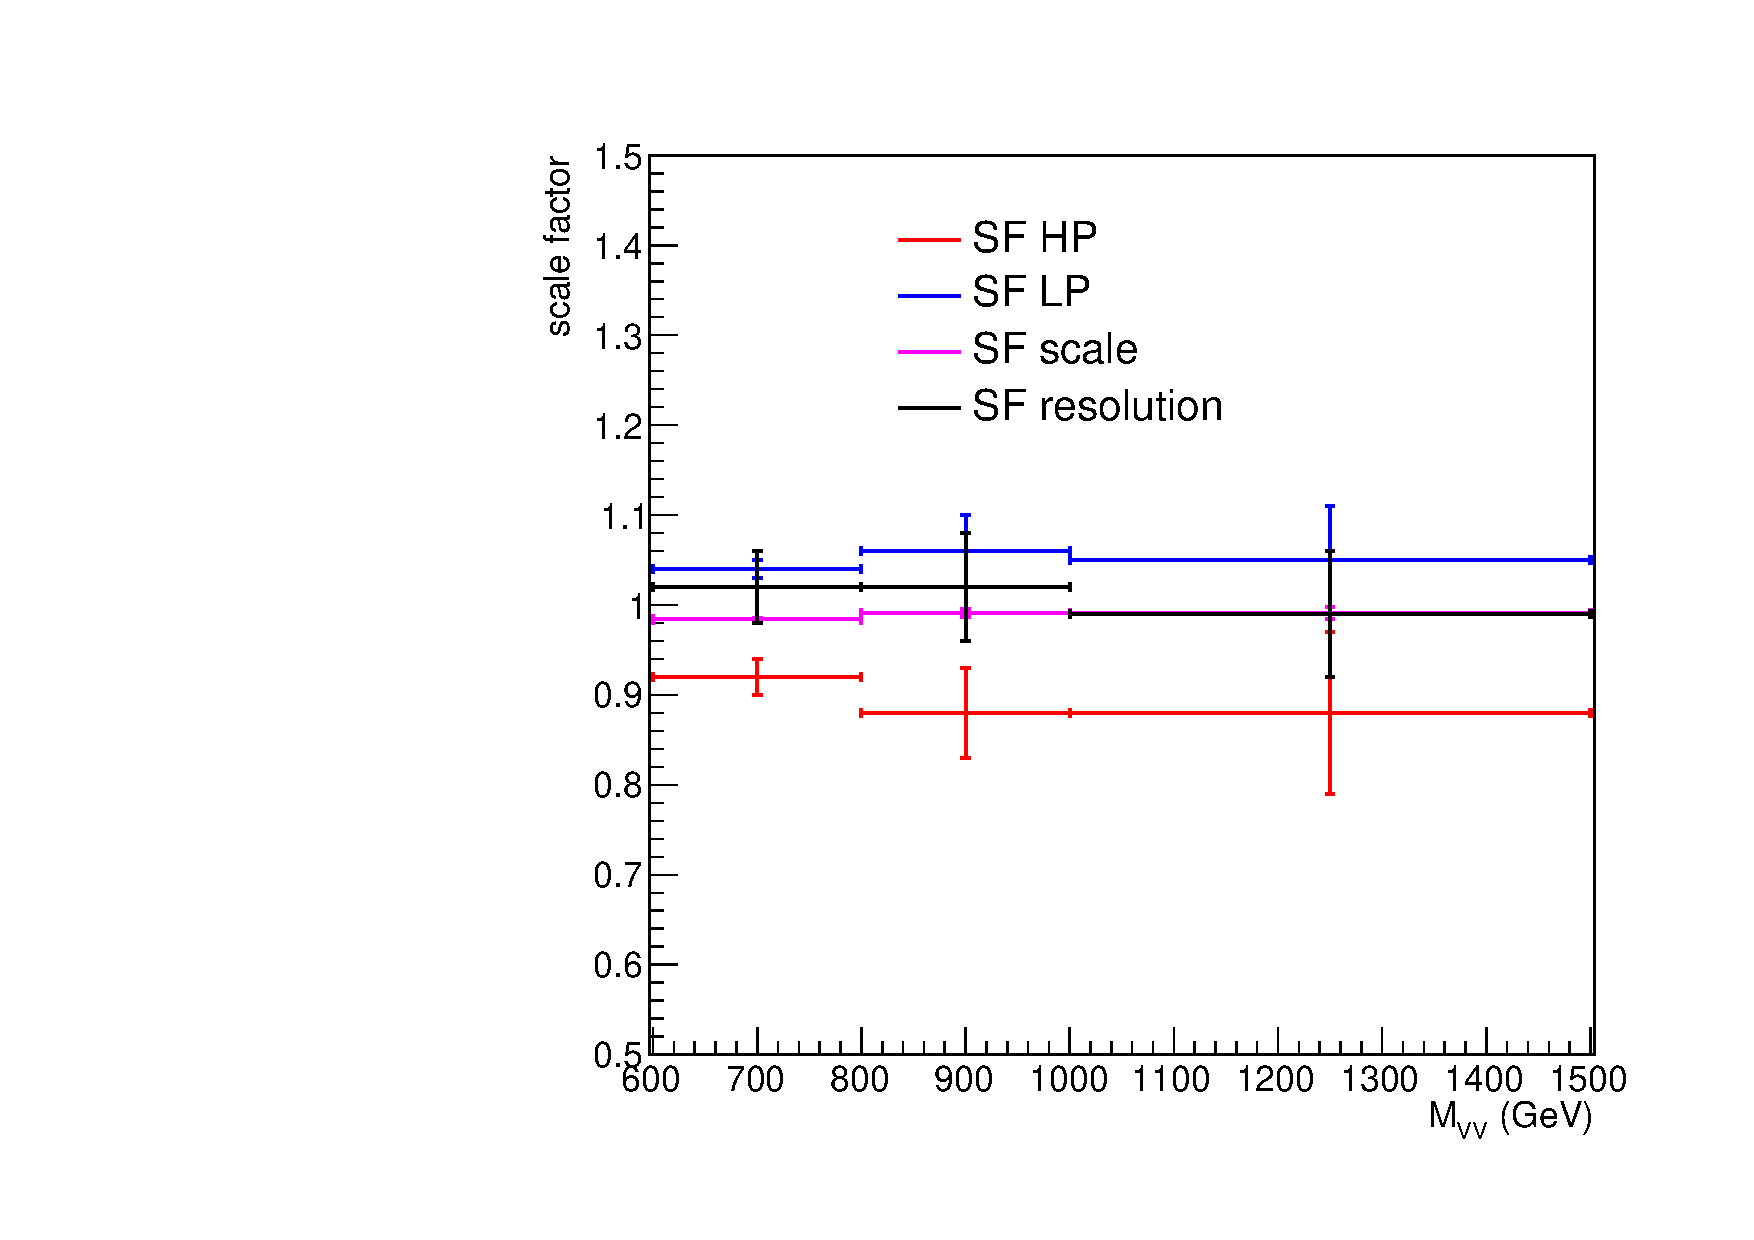
\includegraphics[width=0.45\textwidth]{fig/Vtag/MVVDepSummary.pdf}
  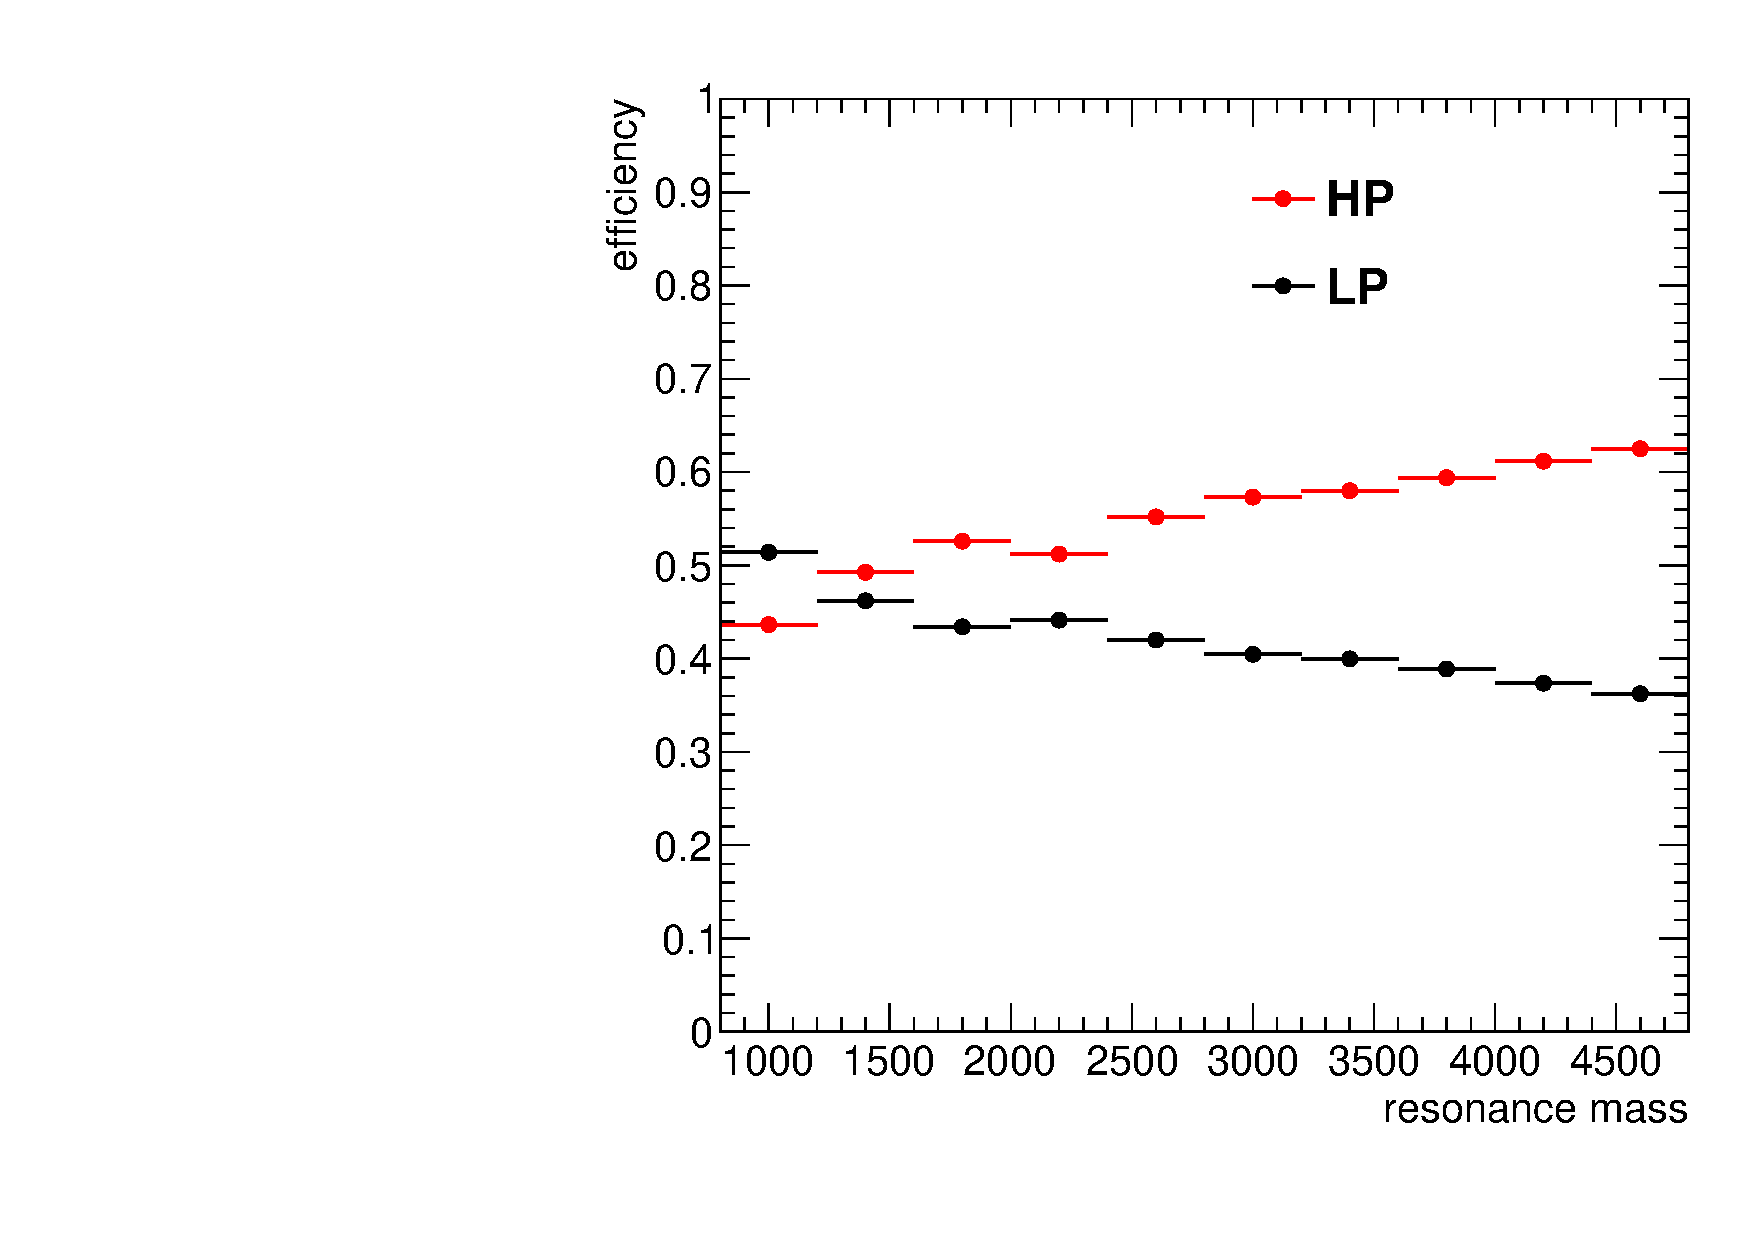
\includegraphics[width=0.45\textwidth]{fig/Vtag/ptDep.pdf}
  \caption{
    Left: Plot of all scale factors as a function of the diboson invariant mass \MVV.
    Right: Plot of the $V$-tagging efficiency as a function of \MVV.
  }
  \label{fig:VTag_massdep_summary}
\end{figure}
